\documentclass[twoside]{book}

% Packages required by doxygen
\usepackage{fixltx2e}
\usepackage{calc}
\usepackage{doxygen}
\usepackage[export]{adjustbox} % also loads graphicx
\usepackage{graphicx}
\usepackage[utf8]{inputenc}
\usepackage{makeidx}
\usepackage{multicol}
\usepackage{multirow}
\PassOptionsToPackage{warn}{textcomp}
\usepackage{textcomp}
\usepackage[nointegrals]{wasysym}
\usepackage[table]{xcolor}

% Font selection
\usepackage[T1]{fontenc}
\usepackage[scaled=.90]{helvet}
\usepackage{courier}
\usepackage{amssymb}
\usepackage{sectsty}
\renewcommand{\familydefault}{\sfdefault}
\allsectionsfont{%
  \fontseries{bc}\selectfont%
  \color{darkgray}%
}
\renewcommand{\DoxyLabelFont}{%
  \fontseries{bc}\selectfont%
  \color{darkgray}%
}
\newcommand{\+}{\discretionary{\mbox{\scriptsize$\hookleftarrow$}}{}{}}

% Page & text layout
\usepackage{geometry}
\geometry{%
  a4paper,%
  top=2.5cm,%
  bottom=2.5cm,%
  left=2.5cm,%
  right=2.5cm%
}
\tolerance=750
\hfuzz=15pt
\hbadness=750
\setlength{\emergencystretch}{15pt}
\setlength{\parindent}{0cm}
\setlength{\parskip}{3ex plus 2ex minus 2ex}
\makeatletter
\renewcommand{\paragraph}{%
  \@startsection{paragraph}{4}{0ex}{-1.0ex}{1.0ex}{%
    \normalfont\normalsize\bfseries\SS@parafont%
  }%
}
\renewcommand{\subparagraph}{%
  \@startsection{subparagraph}{5}{0ex}{-1.0ex}{1.0ex}{%
    \normalfont\normalsize\bfseries\SS@subparafont%
  }%
}
\makeatother

% Headers & footers
\usepackage{fancyhdr}
\pagestyle{fancyplain}
\fancyhead[LE]{\fancyplain{}{\bfseries\thepage}}
\fancyhead[CE]{\fancyplain{}{}}
\fancyhead[RE]{\fancyplain{}{\bfseries\leftmark}}
\fancyhead[LO]{\fancyplain{}{\bfseries\rightmark}}
\fancyhead[CO]{\fancyplain{}{}}
\fancyhead[RO]{\fancyplain{}{\bfseries\thepage}}
\fancyfoot[LE]{\fancyplain{}{}}
\fancyfoot[CE]{\fancyplain{}{}}
\fancyfoot[RE]{\fancyplain{}{\bfseries\scriptsize Generated by Doxygen }}
\fancyfoot[LO]{\fancyplain{}{\bfseries\scriptsize Generated by Doxygen }}
\fancyfoot[CO]{\fancyplain{}{}}
\fancyfoot[RO]{\fancyplain{}{}}
\renewcommand{\footrulewidth}{0.4pt}
\renewcommand{\chaptermark}[1]{%
  \markboth{#1}{}%
}
\renewcommand{\sectionmark}[1]{%
  \markright{\thesection\ #1}%
}

% Indices & bibliography
\usepackage{natbib}
\usepackage[titles]{tocloft}
\setcounter{tocdepth}{3}
\setcounter{secnumdepth}{5}
\makeindex

% Hyperlinks (required, but should be loaded last)
\usepackage{ifpdf}
\ifpdf
  \usepackage[pdftex,pagebackref=true]{hyperref}
\else
  \usepackage[ps2pdf,pagebackref=true]{hyperref}
\fi
\hypersetup{%
  colorlinks=true,%
  linkcolor=blue,%
  citecolor=blue,%
  unicode%
}

% Custom commands
\newcommand{\clearemptydoublepage}{%
  \newpage{\pagestyle{empty}\cleardoublepage}%
}

\usepackage{caption}
\captionsetup{labelsep=space,justification=centering,font={bf},singlelinecheck=off,skip=4pt,position=top}

%===== C O N T E N T S =====

\begin{document}

% Titlepage & ToC
\hypersetup{pageanchor=false,
             bookmarksnumbered=true,
             pdfencoding=unicode
            }
\pagenumbering{alph}
\begin{titlepage}
\vspace*{7cm}
\begin{center}%
{\Large Angry\+U\+ML }\\
\vspace*{1cm}
{\large Generated by Doxygen 1.8.12}\\
\end{center}
\end{titlepage}
\clearemptydoublepage
\pagenumbering{roman}
\tableofcontents
\clearemptydoublepage
\pagenumbering{arabic}
\hypersetup{pageanchor=true}

%--- Begin generated contents ---
\chapter{Namespace Index}
\section{Namespace List}
Here is a list of all documented namespaces with brief descriptions\+:\begin{DoxyCompactList}
\item\contentsline{section}{\hyperlink{namespaceACM_1_1CPP}{A\+C\+M\+::\+C\+PP} }{\pageref{namespaceACM_1_1CPP}}{}
\end{DoxyCompactList}

\chapter{Hierarchical Index}
\section{Class Hierarchy}
This inheritance list is sorted roughly, but not completely, alphabetically\+:\begin{DoxyCompactList}
\item b2\+Contact\+Listener\begin{DoxyCompactList}
\item \contentsline{section}{Collision\+Listener}{\pageref{classCollisionListener}}{}
\end{DoxyCompactList}
\item \contentsline{section}{Item\+Data}{\pageref{classItemData}}{}
\item Q\+Graphics\+Pixmap\+Item\begin{DoxyCompactList}
\item \contentsline{section}{Game\+Engine}{\pageref{classGameEngine}}{}
\item \contentsline{section}{Game\+Item}{\pageref{classGameItem}}{}
\begin{DoxyCompactList}
\item \contentsline{section}{Abs\+Bird}{\pageref{classAbsBird}}{}
\begin{DoxyCompactList}
\item \contentsline{section}{Big\+Bird}{\pageref{classBigBird}}{}
\item \contentsline{section}{Blue\+Bird}{\pageref{classBlueBird}}{}
\item \contentsline{section}{Red\+Bird}{\pageref{classRedBird}}{}
\item \contentsline{section}{Yellow\+Bird}{\pageref{classYellowBird}}{}
\end{DoxyCompactList}
\item \contentsline{section}{Block\+\_\+\+Vtl}{\pageref{classBlock__Vtl}}{}
\item \contentsline{section}{Ground}{\pageref{classGround}}{}
\item \contentsline{section}{Pig1}{\pageref{classPig1}}{}
\item \contentsline{section}{Stick2\+\_\+\+Hrz}{\pageref{classStick2__Hrz}}{}
\item \contentsline{section}{Stick2\+\_\+\+Vtl}{\pageref{classStick2__Vtl}}{}
\item \contentsline{section}{Stick\+\_\+\+Hrz}{\pageref{classStick__Hrz}}{}
\item \contentsline{section}{Stick\+\_\+\+Vtl}{\pageref{classStick__Vtl}}{}
\end{DoxyCompactList}
\item \contentsline{section}{Leave\+Button}{\pageref{classLeaveButton}}{}
\item \contentsline{section}{Restart\+Button}{\pageref{classRestartButton}}{}
\item \contentsline{section}{Singleshot}{\pageref{classSingleshot}}{}
\end{DoxyCompactList}
\item Q\+Graphics\+Scene\begin{DoxyCompactList}
\item \contentsline{section}{End\+Menu\+Scene}{\pageref{classEndMenuScene}}{}
\item \contentsline{section}{Game\+Scene}{\pageref{classGameScene}}{}
\end{DoxyCompactList}
\item Q\+Graphics\+Text\+Item\begin{DoxyCompactList}
\item \contentsline{section}{Bird\+Used\+Amount}{\pageref{classBirdUsedAmount}}{}
\item \contentsline{section}{End\+Score}{\pageref{classEndScore}}{}
\item \contentsline{section}{Play\+Score}{\pageref{classPlayScore}}{}
\end{DoxyCompactList}
\item Q\+Graphics\+View\begin{DoxyCompactList}
\item \contentsline{section}{Game\+View}{\pageref{classGameView}}{}
\end{DoxyCompactList}
\item Q\+Main\+Window\begin{DoxyCompactList}
\item \contentsline{section}{Main\+Window}{\pageref{classMainWindow}}{}
\end{DoxyCompactList}
\item Q\+Object\begin{DoxyCompactList}
\item \contentsline{section}{Collision\+Listener}{\pageref{classCollisionListener}}{}
\item \contentsline{section}{Game\+Engine}{\pageref{classGameEngine}}{}
\item \contentsline{section}{Game\+Item}{\pageref{classGameItem}}{}
\item \contentsline{section}{Leave\+Button}{\pageref{classLeaveButton}}{}
\item \contentsline{section}{Restart\+Button}{\pageref{classRestartButton}}{}
\item \contentsline{section}{Singleshot}{\pageref{classSingleshot}}{}
\end{DoxyCompactList}
\item \contentsline{section}{qt\+\_\+meta\+\_\+stringdata\+\_\+\+Abs\+Bird\+\_\+t}{\pageref{structqt__meta__stringdata__AbsBird__t}}{}
\item \contentsline{section}{qt\+\_\+meta\+\_\+stringdata\+\_\+\+Big\+Bird\+\_\+t}{\pageref{structqt__meta__stringdata__BigBird__t}}{}
\item \contentsline{section}{qt\+\_\+meta\+\_\+stringdata\+\_\+\+Bird\+Used\+Amount\+\_\+t}{\pageref{structqt__meta__stringdata__BirdUsedAmount__t}}{}
\item \contentsline{section}{qt\+\_\+meta\+\_\+stringdata\+\_\+\+Block\+\_\+\+Vtl\+\_\+t}{\pageref{structqt__meta__stringdata__Block__Vtl__t}}{}
\item \contentsline{section}{qt\+\_\+meta\+\_\+stringdata\+\_\+\+Blue\+Bird\+\_\+t}{\pageref{structqt__meta__stringdata__BlueBird__t}}{}
\item \contentsline{section}{qt\+\_\+meta\+\_\+stringdata\+\_\+\+Collision\+Listener\+\_\+t}{\pageref{structqt__meta__stringdata__CollisionListener__t}}{}
\item \contentsline{section}{qt\+\_\+meta\+\_\+stringdata\+\_\+\+End\+Score\+\_\+t}{\pageref{structqt__meta__stringdata__EndScore__t}}{}
\item \contentsline{section}{qt\+\_\+meta\+\_\+stringdata\+\_\+\+Game\+Engine\+\_\+t}{\pageref{structqt__meta__stringdata__GameEngine__t}}{}
\item \contentsline{section}{qt\+\_\+meta\+\_\+stringdata\+\_\+\+Game\+Item\+\_\+t}{\pageref{structqt__meta__stringdata__GameItem__t}}{}
\item \contentsline{section}{qt\+\_\+meta\+\_\+stringdata\+\_\+\+Game\+Scene\+\_\+t}{\pageref{structqt__meta__stringdata__GameScene__t}}{}
\item \contentsline{section}{qt\+\_\+meta\+\_\+stringdata\+\_\+\+Game\+View\+\_\+t}{\pageref{structqt__meta__stringdata__GameView__t}}{}
\item \contentsline{section}{qt\+\_\+meta\+\_\+stringdata\+\_\+\+Leave\+Button\+\_\+t}{\pageref{structqt__meta__stringdata__LeaveButton__t}}{}
\item \contentsline{section}{qt\+\_\+meta\+\_\+stringdata\+\_\+\+Main\+Window\+\_\+t}{\pageref{structqt__meta__stringdata__MainWindow__t}}{}
\item \contentsline{section}{qt\+\_\+meta\+\_\+stringdata\+\_\+\+Pig1\+\_\+t}{\pageref{structqt__meta__stringdata__Pig1__t}}{}
\item \contentsline{section}{qt\+\_\+meta\+\_\+stringdata\+\_\+\+Play\+Score\+\_\+t}{\pageref{structqt__meta__stringdata__PlayScore__t}}{}
\item \contentsline{section}{qt\+\_\+meta\+\_\+stringdata\+\_\+\+Red\+Bird\+\_\+t}{\pageref{structqt__meta__stringdata__RedBird__t}}{}
\item \contentsline{section}{qt\+\_\+meta\+\_\+stringdata\+\_\+\+Restart\+Button\+\_\+t}{\pageref{structqt__meta__stringdata__RestartButton__t}}{}
\item \contentsline{section}{qt\+\_\+meta\+\_\+stringdata\+\_\+\+Singleshot\+\_\+t}{\pageref{structqt__meta__stringdata__Singleshot__t}}{}
\item \contentsline{section}{qt\+\_\+meta\+\_\+stringdata\+\_\+\+Stick2\+\_\+\+Hrz\+\_\+t}{\pageref{structqt__meta__stringdata__Stick2__Hrz__t}}{}
\item \contentsline{section}{qt\+\_\+meta\+\_\+stringdata\+\_\+\+Stick2\+\_\+\+Vtl\+\_\+t}{\pageref{structqt__meta__stringdata__Stick2__Vtl__t}}{}
\item \contentsline{section}{qt\+\_\+meta\+\_\+stringdata\+\_\+\+Stick\+\_\+\+Hrz\+\_\+t}{\pageref{structqt__meta__stringdata__Stick__Hrz__t}}{}
\item \contentsline{section}{qt\+\_\+meta\+\_\+stringdata\+\_\+\+Stick\+\_\+t}{\pageref{structqt__meta__stringdata__Stick__t}}{}
\item \contentsline{section}{qt\+\_\+meta\+\_\+stringdata\+\_\+\+Stick\+\_\+\+Vtl\+\_\+t}{\pageref{structqt__meta__stringdata__Stick__Vtl__t}}{}
\item \contentsline{section}{qt\+\_\+meta\+\_\+stringdata\+\_\+\+Yellow\+Bird\+\_\+t}{\pageref{structqt__meta__stringdata__YellowBird__t}}{}
\end{DoxyCompactList}

\chapter{Class Index}
\section{Class List}
Here are the classes, structs, unions and interfaces with brief descriptions\+:\begin{DoxyCompactList}
\item\contentsline{section}{\hyperlink{classAbsBird}{Abs\+Bird} }{\pageref{classAbsBird}}{}
\item\contentsline{section}{\hyperlink{classBigBird}{Big\+Bird} }{\pageref{classBigBird}}{}
\item\contentsline{section}{\hyperlink{classBirdUsedAmount}{Bird\+Used\+Amount} }{\pageref{classBirdUsedAmount}}{}
\item\contentsline{section}{\hyperlink{classBlock__Vtl}{Block\+\_\+\+Vtl} }{\pageref{classBlock__Vtl}}{}
\item\contentsline{section}{\hyperlink{classBlueBird}{Blue\+Bird} }{\pageref{classBlueBird}}{}
\item\contentsline{section}{\hyperlink{classCollisionListener}{Collision\+Listener} }{\pageref{classCollisionListener}}{}
\item\contentsline{section}{\hyperlink{classEndMenuScene}{End\+Menu\+Scene} }{\pageref{classEndMenuScene}}{}
\item\contentsline{section}{\hyperlink{classEndScore}{End\+Score} }{\pageref{classEndScore}}{}
\item\contentsline{section}{\hyperlink{classGameEngine}{Game\+Engine} }{\pageref{classGameEngine}}{}
\item\contentsline{section}{\hyperlink{classGameItem}{Game\+Item} }{\pageref{classGameItem}}{}
\item\contentsline{section}{\hyperlink{classGameScene}{Game\+Scene} }{\pageref{classGameScene}}{}
\item\contentsline{section}{\hyperlink{classGameView}{Game\+View} }{\pageref{classGameView}}{}
\item\contentsline{section}{\hyperlink{classGround}{Ground} }{\pageref{classGround}}{}
\item\contentsline{section}{\hyperlink{classItemData}{Item\+Data} }{\pageref{classItemData}}{}
\item\contentsline{section}{\hyperlink{classLeaveButton}{Leave\+Button} }{\pageref{classLeaveButton}}{}
\item\contentsline{section}{\hyperlink{classMainWindow}{Main\+Window} }{\pageref{classMainWindow}}{}
\item\contentsline{section}{\hyperlink{classPig1}{Pig1} }{\pageref{classPig1}}{}
\item\contentsline{section}{\hyperlink{classPlayScore}{Play\+Score} }{\pageref{classPlayScore}}{}
\item\contentsline{section}{\hyperlink{structqt__meta__stringdata__AbsBird__t}{qt\+\_\+meta\+\_\+stringdata\+\_\+\+Abs\+Bird\+\_\+t} }{\pageref{structqt__meta__stringdata__AbsBird__t}}{}
\item\contentsline{section}{\hyperlink{structqt__meta__stringdata__BigBird__t}{qt\+\_\+meta\+\_\+stringdata\+\_\+\+Big\+Bird\+\_\+t} }{\pageref{structqt__meta__stringdata__BigBird__t}}{}
\item\contentsline{section}{\hyperlink{structqt__meta__stringdata__BirdUsedAmount__t}{qt\+\_\+meta\+\_\+stringdata\+\_\+\+Bird\+Used\+Amount\+\_\+t} }{\pageref{structqt__meta__stringdata__BirdUsedAmount__t}}{}
\item\contentsline{section}{\hyperlink{structqt__meta__stringdata__Block__Vtl__t}{qt\+\_\+meta\+\_\+stringdata\+\_\+\+Block\+\_\+\+Vtl\+\_\+t} }{\pageref{structqt__meta__stringdata__Block__Vtl__t}}{}
\item\contentsline{section}{\hyperlink{structqt__meta__stringdata__BlueBird__t}{qt\+\_\+meta\+\_\+stringdata\+\_\+\+Blue\+Bird\+\_\+t} }{\pageref{structqt__meta__stringdata__BlueBird__t}}{}
\item\contentsline{section}{\hyperlink{structqt__meta__stringdata__CollisionListener__t}{qt\+\_\+meta\+\_\+stringdata\+\_\+\+Collision\+Listener\+\_\+t} }{\pageref{structqt__meta__stringdata__CollisionListener__t}}{}
\item\contentsline{section}{\hyperlink{structqt__meta__stringdata__EndScore__t}{qt\+\_\+meta\+\_\+stringdata\+\_\+\+End\+Score\+\_\+t} }{\pageref{structqt__meta__stringdata__EndScore__t}}{}
\item\contentsline{section}{\hyperlink{structqt__meta__stringdata__GameEngine__t}{qt\+\_\+meta\+\_\+stringdata\+\_\+\+Game\+Engine\+\_\+t} }{\pageref{structqt__meta__stringdata__GameEngine__t}}{}
\item\contentsline{section}{\hyperlink{structqt__meta__stringdata__GameItem__t}{qt\+\_\+meta\+\_\+stringdata\+\_\+\+Game\+Item\+\_\+t} }{\pageref{structqt__meta__stringdata__GameItem__t}}{}
\item\contentsline{section}{\hyperlink{structqt__meta__stringdata__GameScene__t}{qt\+\_\+meta\+\_\+stringdata\+\_\+\+Game\+Scene\+\_\+t} }{\pageref{structqt__meta__stringdata__GameScene__t}}{}
\item\contentsline{section}{\hyperlink{structqt__meta__stringdata__GameView__t}{qt\+\_\+meta\+\_\+stringdata\+\_\+\+Game\+View\+\_\+t} }{\pageref{structqt__meta__stringdata__GameView__t}}{}
\item\contentsline{section}{\hyperlink{structqt__meta__stringdata__LeaveButton__t}{qt\+\_\+meta\+\_\+stringdata\+\_\+\+Leave\+Button\+\_\+t} }{\pageref{structqt__meta__stringdata__LeaveButton__t}}{}
\item\contentsline{section}{\hyperlink{structqt__meta__stringdata__MainWindow__t}{qt\+\_\+meta\+\_\+stringdata\+\_\+\+Main\+Window\+\_\+t} }{\pageref{structqt__meta__stringdata__MainWindow__t}}{}
\item\contentsline{section}{\hyperlink{structqt__meta__stringdata__Pig1__t}{qt\+\_\+meta\+\_\+stringdata\+\_\+\+Pig1\+\_\+t} }{\pageref{structqt__meta__stringdata__Pig1__t}}{}
\item\contentsline{section}{\hyperlink{structqt__meta__stringdata__PlayScore__t}{qt\+\_\+meta\+\_\+stringdata\+\_\+\+Play\+Score\+\_\+t} }{\pageref{structqt__meta__stringdata__PlayScore__t}}{}
\item\contentsline{section}{\hyperlink{structqt__meta__stringdata__RedBird__t}{qt\+\_\+meta\+\_\+stringdata\+\_\+\+Red\+Bird\+\_\+t} }{\pageref{structqt__meta__stringdata__RedBird__t}}{}
\item\contentsline{section}{\hyperlink{structqt__meta__stringdata__RestartButton__t}{qt\+\_\+meta\+\_\+stringdata\+\_\+\+Restart\+Button\+\_\+t} }{\pageref{structqt__meta__stringdata__RestartButton__t}}{}
\item\contentsline{section}{\hyperlink{structqt__meta__stringdata__Singleshot__t}{qt\+\_\+meta\+\_\+stringdata\+\_\+\+Singleshot\+\_\+t} }{\pageref{structqt__meta__stringdata__Singleshot__t}}{}
\item\contentsline{section}{\hyperlink{structqt__meta__stringdata__Stick2__Hrz__t}{qt\+\_\+meta\+\_\+stringdata\+\_\+\+Stick2\+\_\+\+Hrz\+\_\+t} }{\pageref{structqt__meta__stringdata__Stick2__Hrz__t}}{}
\item\contentsline{section}{\hyperlink{structqt__meta__stringdata__Stick2__Vtl__t}{qt\+\_\+meta\+\_\+stringdata\+\_\+\+Stick2\+\_\+\+Vtl\+\_\+t} }{\pageref{structqt__meta__stringdata__Stick2__Vtl__t}}{}
\item\contentsline{section}{\hyperlink{structqt__meta__stringdata__Stick__Hrz__t}{qt\+\_\+meta\+\_\+stringdata\+\_\+\+Stick\+\_\+\+Hrz\+\_\+t} }{\pageref{structqt__meta__stringdata__Stick__Hrz__t}}{}
\item\contentsline{section}{\hyperlink{structqt__meta__stringdata__Stick__t}{qt\+\_\+meta\+\_\+stringdata\+\_\+\+Stick\+\_\+t} }{\pageref{structqt__meta__stringdata__Stick__t}}{}
\item\contentsline{section}{\hyperlink{structqt__meta__stringdata__Stick__Vtl__t}{qt\+\_\+meta\+\_\+stringdata\+\_\+\+Stick\+\_\+\+Vtl\+\_\+t} }{\pageref{structqt__meta__stringdata__Stick__Vtl__t}}{}
\item\contentsline{section}{\hyperlink{structqt__meta__stringdata__YellowBird__t}{qt\+\_\+meta\+\_\+stringdata\+\_\+\+Yellow\+Bird\+\_\+t} }{\pageref{structqt__meta__stringdata__YellowBird__t}}{}
\item\contentsline{section}{\hyperlink{classRedBird}{Red\+Bird} }{\pageref{classRedBird}}{}
\item\contentsline{section}{\hyperlink{classRestartButton}{Restart\+Button} }{\pageref{classRestartButton}}{}
\item\contentsline{section}{\hyperlink{classSingleshot}{Singleshot} }{\pageref{classSingleshot}}{}
\item\contentsline{section}{\hyperlink{classStick2__Hrz}{Stick2\+\_\+\+Hrz} }{\pageref{classStick2__Hrz}}{}
\item\contentsline{section}{\hyperlink{classStick2__Vtl}{Stick2\+\_\+\+Vtl} }{\pageref{classStick2__Vtl}}{}
\item\contentsline{section}{\hyperlink{classStick__Hrz}{Stick\+\_\+\+Hrz} }{\pageref{classStick__Hrz}}{}
\item\contentsline{section}{\hyperlink{classStick__Vtl}{Stick\+\_\+\+Vtl} }{\pageref{classStick__Vtl}}{}
\item\contentsline{section}{\hyperlink{classYellowBird}{Yellow\+Bird} }{\pageref{classYellowBird}}{}
\end{DoxyCompactList}

\chapter{Namespace Documentation}
\hypertarget{namespaceACM_1_1CPP}{}\section{A\+CM\+:\+:C\+PP Namespace Reference}
\label{namespaceACM_1_1CPP}\index{A\+C\+M\+::\+C\+PP@{A\+C\+M\+::\+C\+PP}}
\subsection*{Functions}
\begin{DoxyCompactItemize}
\item 
\hyperlink{namespaceACM_1_1CPP_a8fe11d3a728c1a7fc3c77b199cdb6603}{get\+Next\+Token} pline pindex ptype args
\end{DoxyCompactItemize}


\subsection{Detailed Description}
\subparagraph*{}

get\+Next\+Token 
\begin{DoxyParams}{Parameters}
{\em pline} & variable name of linenumber \\
\hline
{\em pindex} & variable name of column in line \\
\hline
{\em ptype} & variable name of type buffer \\
\hline
\end{DoxyParams}
\begin{DoxyReturn}{Returns}
content of token ptype will contain one of ( W\+O\+RD, K\+E\+Y\+W\+O\+RD, N\+U\+M\+B\+ER, P\+R\+EP, M\+I\+SC ) 
\end{DoxyReturn}


\subsection{Function Documentation}
\index{A\+C\+M\+::\+C\+PP@{A\+C\+M\+::\+C\+PP}!get\+Next\+Token@{get\+Next\+Token}}
\index{get\+Next\+Token@{get\+Next\+Token}!A\+C\+M\+::\+C\+PP@{A\+C\+M\+::\+C\+PP}}
\subsubsection[{\texorpdfstring{get\+Next\+Tokenpline pindex ptype args}{getNextTokenpline pindex ptype args}}]{\setlength{\rightskip}{0pt plus 5cm}A\+C\+M\+::\+C\+P\+P\+::get\+Next\+Token
\begin{DoxyParamCaption}
\item[{}]{pline pindex ptype args }
\end{DoxyParamCaption}
}\hypertarget{namespaceACM_1_1CPP_a8fe11d3a728c1a7fc3c77b199cdb6603}{}\label{namespaceACM_1_1CPP_a8fe11d3a728c1a7fc3c77b199cdb6603}
\subparagraph*{}
\chapter{Class Documentation}
\hypertarget{classAbsBird}{}\section{Abs\+Bird Class Reference}
\label{classAbsBird}\index{Abs\+Bird@{Abs\+Bird}}
Inheritance diagram for Abs\+Bird\+:\begin{figure}[H]
\begin{center}
\leavevmode
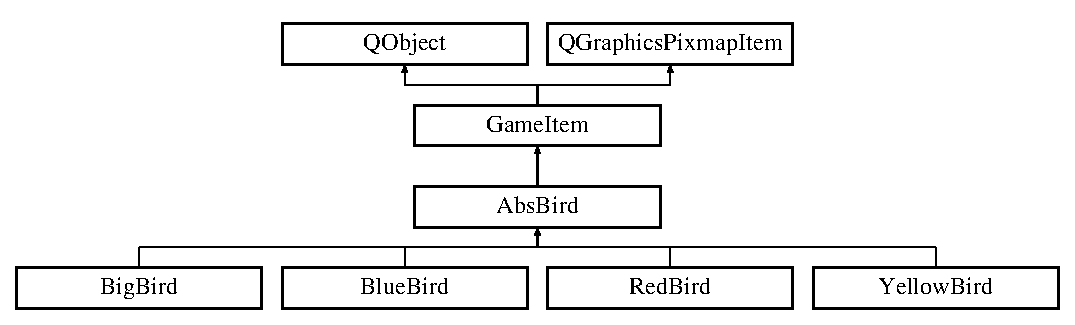
\includegraphics[height=3.916084cm]{classAbsBird}
\end{center}
\end{figure}
\subsection*{Public Slots}
\begin{DoxyCompactItemize}
\item 
virtual void {\bfseries set\+Pull\+Pos} (int x, int y)\hypertarget{classAbsBird_a82b0185bc20c859c92321ff849d27020}{}\label{classAbsBird_a82b0185bc20c859c92321ff849d27020}

\item 
void {\bfseries update\+Pos} ()\hypertarget{classAbsBird_a360c1ee1844ceee60625dad148bf3d49}{}\label{classAbsBird_a360c1ee1844ceee60625dad148bf3d49}

\item 
virtual void {\bfseries special\+Ability} ()\hypertarget{classAbsBird_a83c7cf1a8deda52d57f3b79662b9a03e}{}\label{classAbsBird_a83c7cf1a8deda52d57f3b79662b9a03e}

\item 
void {\bfseries release\+Bird} (int forceX, int forceY)\hypertarget{classAbsBird_a6908dc186b792cc4b376f362dab34e92}{}\label{classAbsBird_a6908dc186b792cc4b376f362dab34e92}

\end{DoxyCompactItemize}
\subsection*{Additional Inherited Members}


The documentation for this class was generated from the following files\+:\begin{DoxyCompactItemize}
\item 
Game\+Scene/\+Abs\+Classes/Abs\+Bird.\+h\item 
Game\+Scene/\+Abs\+Classes/Abs\+Bird.\+cpp\end{DoxyCompactItemize}

\hypertarget{classBigBird}{}\section{Big\+Bird Class Reference}
\label{classBigBird}\index{Big\+Bird@{Big\+Bird}}
Inheritance diagram for Big\+Bird\+:\begin{figure}[H]
\begin{center}
\leavevmode
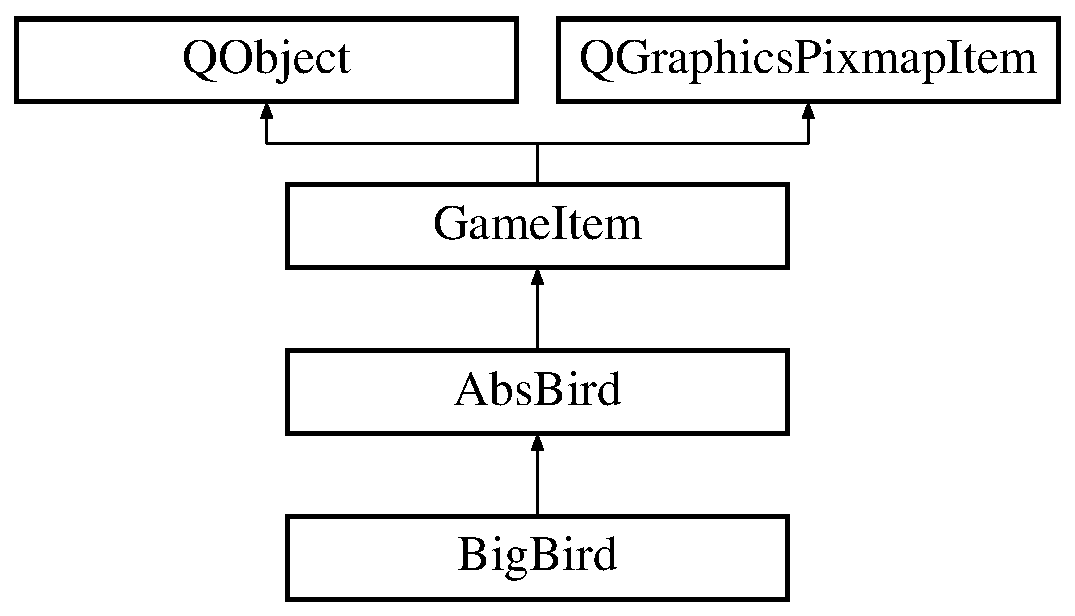
\includegraphics[height=4.000000cm]{classBigBird}
\end{center}
\end{figure}
\subsection*{Public Slots}
\begin{DoxyCompactItemize}
\item 
void {\bfseries set\+Pull\+Pos} (int x, int y)\hypertarget{classBigBird_a323a0647de091d51d04cf8c4cb284d75}{}\label{classBigBird_a323a0647de091d51d04cf8c4cb284d75}

\item 
void {\bfseries update\+Pos} ()\hypertarget{classBigBird_aca8b3e130311603afe47dabdc4af1e27}{}\label{classBigBird_aca8b3e130311603afe47dabdc4af1e27}

\item 
void {\bfseries special\+Ability} ()\hypertarget{classBigBird_a374b32ac67f4e3d1bf0cd05fc5564252}{}\label{classBigBird_a374b32ac67f4e3d1bf0cd05fc5564252}

\end{DoxyCompactItemize}
\subsection*{Public Member Functions}
\begin{DoxyCompactItemize}
\item 
{\bfseries Big\+Bird} (b2\+World $\ast$input\+World)\hypertarget{classBigBird_ab63f9969f3c08fd623a5f9e1e034d18d}{}\label{classBigBird_ab63f9969f3c08fd623a5f9e1e034d18d}

\end{DoxyCompactItemize}
\subsection*{Additional Inherited Members}


The documentation for this class was generated from the following files\+:\begin{DoxyCompactItemize}
\item 
Game\+Scene/\+Birds/Big\+Bird.\+h\item 
Game\+Scene/\+Birds/Big\+Bird.\+cpp\end{DoxyCompactItemize}

\hypertarget{classBirdUsedAmount}{}\section{Bird\+Used\+Amount Class Reference}
\label{classBirdUsedAmount}\index{Bird\+Used\+Amount@{Bird\+Used\+Amount}}
Inheritance diagram for Bird\+Used\+Amount\+:\begin{figure}[H]
\begin{center}
\leavevmode
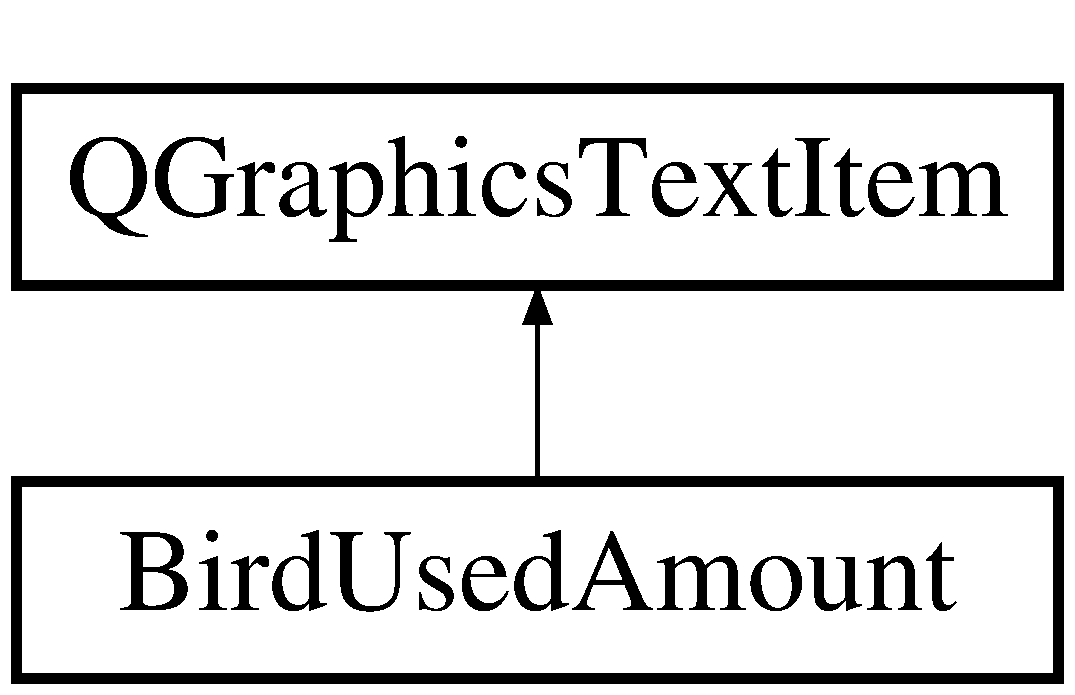
\includegraphics[height=2.000000cm]{classBirdUsedAmount}
\end{center}
\end{figure}
\subsection*{Public Slots}
\begin{DoxyCompactItemize}
\item 
void {\bfseries add\+Amount} ()\hypertarget{classBirdUsedAmount_ac64d566977df6e370b204ab06db6a574}{}\label{classBirdUsedAmount_ac64d566977df6e370b204ab06db6a574}

\end{DoxyCompactItemize}
\subsection*{Public Member Functions}
\begin{DoxyCompactItemize}
\item 
{\bfseries Bird\+Used\+Amount} (int input\+Amount)\hypertarget{classBirdUsedAmount_a42811d8fbbfef7780cc105e30c75fa0f}{}\label{classBirdUsedAmount_a42811d8fbbfef7780cc105e30c75fa0f}

\end{DoxyCompactItemize}
\subsection*{Public Attributes}
\begin{DoxyCompactItemize}
\item 
int {\bfseries used\+Amount}\hypertarget{classBirdUsedAmount_a76196a8af37a37e1b19135b404691517}{}\label{classBirdUsedAmount_a76196a8af37a37e1b19135b404691517}

\item 
int {\bfseries run}\hypertarget{classBirdUsedAmount_a7351cd1c0f03c21b1e8dfd0400949781}{}\label{classBirdUsedAmount_a7351cd1c0f03c21b1e8dfd0400949781}

\item 
Q\+Timer $\ast$ {\bfseries add\+Timer}\hypertarget{classBirdUsedAmount_a951a7f66b32e664e18cbf569dd6e22c6}{}\label{classBirdUsedAmount_a951a7f66b32e664e18cbf569dd6e22c6}

\end{DoxyCompactItemize}


The documentation for this class was generated from the following files\+:\begin{DoxyCompactItemize}
\item 
End\+Menu\+Scene/Bird\+Used\+Amount.\+h\item 
End\+Menu\+Scene/Bird\+Used\+Amount.\+cpp\end{DoxyCompactItemize}

\hypertarget{classBlock__Vtl}{}\section{Block\+\_\+\+Vtl Class Reference}
\label{classBlock__Vtl}\index{Block\+\_\+\+Vtl@{Block\+\_\+\+Vtl}}
Inheritance diagram for Block\+\_\+\+Vtl\+:\begin{figure}[H]
\begin{center}
\leavevmode
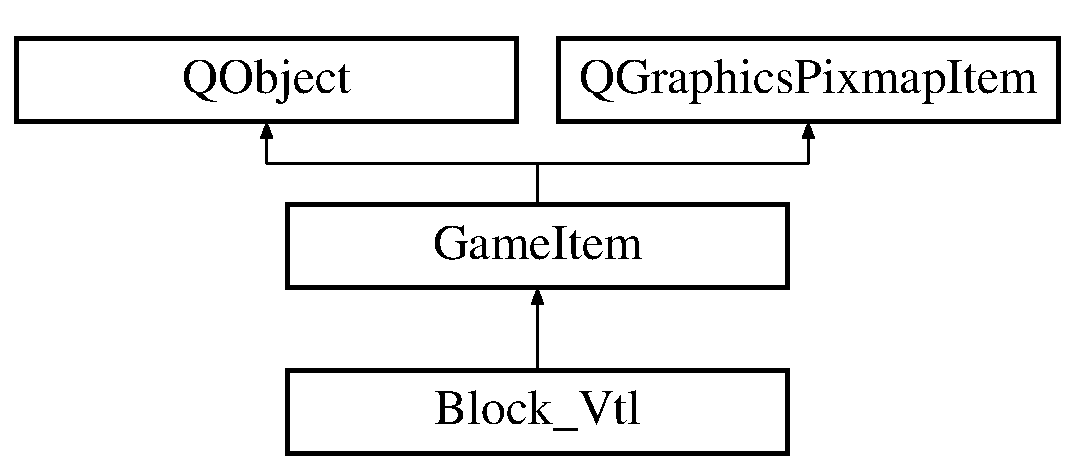
\includegraphics[height=3.000000cm]{classBlock__Vtl}
\end{center}
\end{figure}
\subsection*{Public Member Functions}
\begin{DoxyCompactItemize}
\item 
{\bfseries Block\+\_\+\+Vtl} (b2\+World $\ast$input\+World, int inputX, int inputY)\hypertarget{classBlock__Vtl_ad8c12ec4204968a05785e34f613db275}{}\label{classBlock__Vtl_ad8c12ec4204968a05785e34f613db275}

\end{DoxyCompactItemize}
\subsection*{Additional Inherited Members}


The documentation for this class was generated from the following files\+:\begin{DoxyCompactItemize}
\item 
Game\+Scene/\+Random\+Items/Block\+\_\+\+Vtl.\+h\item 
Game\+Scene/\+Random\+Items/Block\+\_\+\+Vtl.\+cpp\end{DoxyCompactItemize}

\hypertarget{classBlueBird}{}\section{Blue\+Bird Class Reference}
\label{classBlueBird}\index{Blue\+Bird@{Blue\+Bird}}
Inheritance diagram for Blue\+Bird\+:\begin{figure}[H]
\begin{center}
\leavevmode
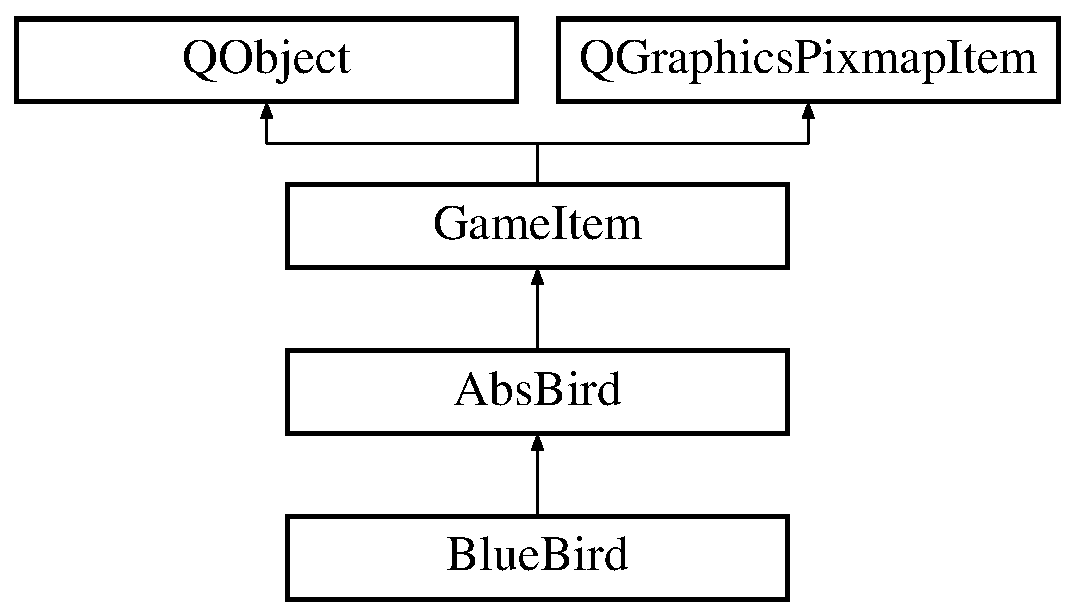
\includegraphics[height=4.000000cm]{classBlueBird}
\end{center}
\end{figure}
\subsection*{Public Slots}
\begin{DoxyCompactItemize}
\item 
void {\bfseries update\+Pos} ()\hypertarget{classBlueBird_a07d51f73da430f56019e507a2b575f62}{}\label{classBlueBird_a07d51f73da430f56019e507a2b575f62}

\item 
void {\bfseries special\+Ability} ()\hypertarget{classBlueBird_afc51650104f6d4572d05d1624e529a1e}{}\label{classBlueBird_afc51650104f6d4572d05d1624e529a1e}

\end{DoxyCompactItemize}
\subsection*{Signals}
\begin{DoxyCompactItemize}
\item 
void {\bfseries spawn\+Blue\+Child} (int x, int y)\hypertarget{classBlueBird_aa4e5f4ce6da8d99c42a10c1cadd2d91c}{}\label{classBlueBird_aa4e5f4ce6da8d99c42a10c1cadd2d91c}

\end{DoxyCompactItemize}
\subsection*{Public Member Functions}
\begin{DoxyCompactItemize}
\item 
{\bfseries Blue\+Bird} (b2\+World $\ast$input\+World, int inputX=0, int inputY=0)\hypertarget{classBlueBird_a8ed2396b0182e8985500d5c672fa3f80}{}\label{classBlueBird_a8ed2396b0182e8985500d5c672fa3f80}

\end{DoxyCompactItemize}
\subsection*{Additional Inherited Members}


The documentation for this class was generated from the following files\+:\begin{DoxyCompactItemize}
\item 
Game\+Scene/\+Birds/Blue\+Bird.\+h\item 
Game\+Scene/\+Birds/Blue\+Bird.\+cpp\item 
moc\+\_\+\+Blue\+Bird.\+cpp\end{DoxyCompactItemize}

\hypertarget{classCollisionListener}{}\section{Collision\+Listener Class Reference}
\label{classCollisionListener}\index{Collision\+Listener@{Collision\+Listener}}
Inheritance diagram for Collision\+Listener\+:\begin{figure}[H]
\begin{center}
\leavevmode
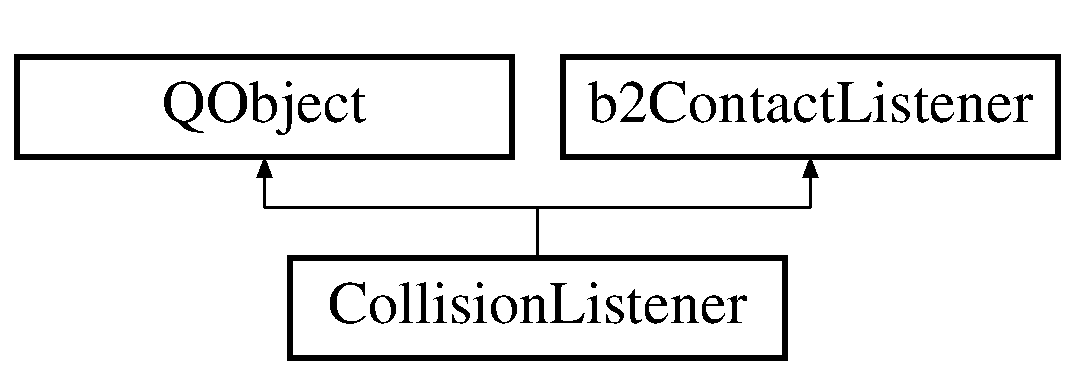
\includegraphics[height=2.000000cm]{classCollisionListener}
\end{center}
\end{figure}
\subsection*{Signals}
\begin{DoxyCompactItemize}
\item 
void {\bfseries spawn\+Score} (int)\hypertarget{classCollisionListener_ab470867a6bd34c86f96e17c393268bef}{}\label{classCollisionListener_ab470867a6bd34c86f96e17c393268bef}

\item 
void {\bfseries kill\+Pig} ()\hypertarget{classCollisionListener_a7de663bb56e4b2a63c8cd605166ec80a}{}\label{classCollisionListener_a7de663bb56e4b2a63c8cd605166ec80a}

\end{DoxyCompactItemize}
\subsection*{Public Member Functions}
\begin{DoxyCompactItemize}
\item 
void {\bfseries Begin\+Contact} (b2\+Contact $\ast$contact)\hypertarget{classCollisionListener_a0d57b91d91ad461f9cc555181209d911}{}\label{classCollisionListener_a0d57b91d91ad461f9cc555181209d911}

\item 
void {\bfseries End\+Contact} (b2\+Contact $\ast$contact)\hypertarget{classCollisionListener_ae1f187fd7825da08d601831534ab57a5}{}\label{classCollisionListener_ae1f187fd7825da08d601831534ab57a5}

\item 
void {\bfseries Pre\+Solve} (b2\+Contact $\ast$contact, const b2\+Manifold $\ast$old\+Manifold)\hypertarget{classCollisionListener_accc6ff23dcbf8cbef31e68fe3c56837a}{}\label{classCollisionListener_accc6ff23dcbf8cbef31e68fe3c56837a}

\item 
void {\bfseries Post\+Solve} (b2\+Contact $\ast$contact, const b2\+Contact\+Impulse $\ast$impulse)\hypertarget{classCollisionListener_a031bc60d472eb4c2996bfc2be6fbc83f}{}\label{classCollisionListener_a031bc60d472eb4c2996bfc2be6fbc83f}

\end{DoxyCompactItemize}


The documentation for this class was generated from the following files\+:\begin{DoxyCompactItemize}
\item 
Game\+Scene/Collision\+Listener.\+h\item 
Game\+Scene/Collision\+Listener.\+cpp\item 
moc\+\_\+\+Collision\+Listener.\+cpp\end{DoxyCompactItemize}

\hypertarget{classEndMenuScene}{}\section{End\+Menu\+Scene Class Reference}
\label{classEndMenuScene}\index{End\+Menu\+Scene@{End\+Menu\+Scene}}
Inheritance diagram for End\+Menu\+Scene\+:\begin{figure}[H]
\begin{center}
\leavevmode
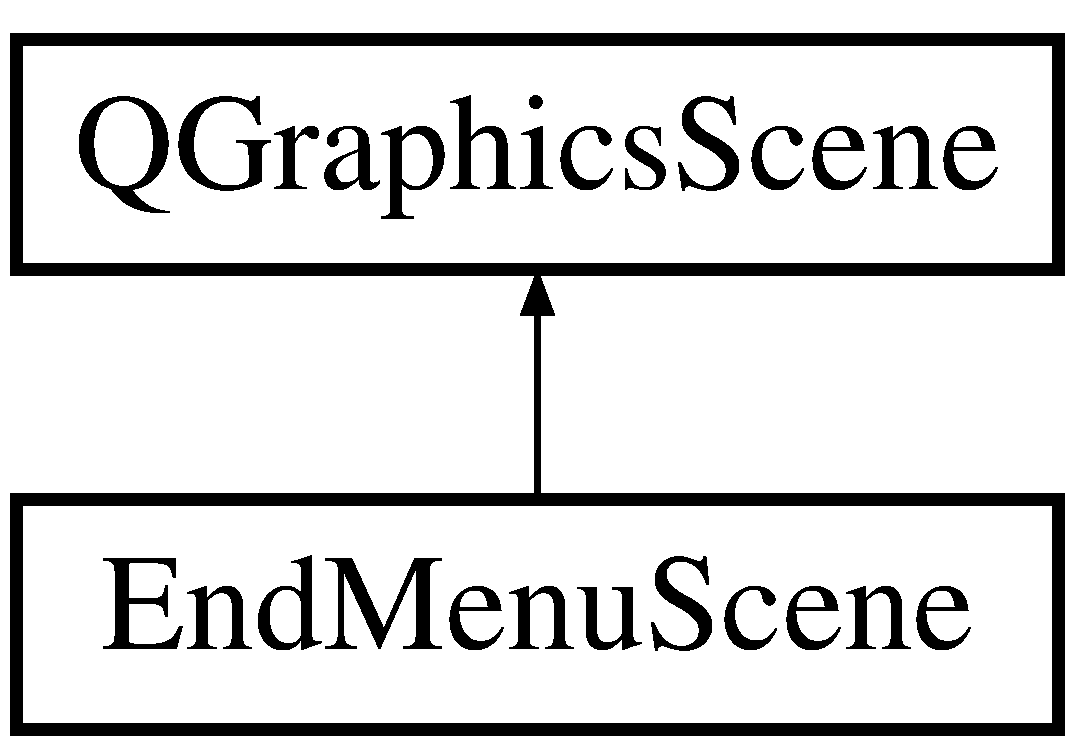
\includegraphics[height=2.000000cm]{classEndMenuScene}
\end{center}
\end{figure}
\subsection*{Public Member Functions}
\begin{DoxyCompactItemize}
\item 
{\bfseries End\+Menu\+Scene} (int score\+Get, int bird\+Used)\hypertarget{classEndMenuScene_a7bf73b3aaae82ec329c8df40b24d7d67}{}\label{classEndMenuScene_a7bf73b3aaae82ec329c8df40b24d7d67}

\end{DoxyCompactItemize}
\subsection*{Public Attributes}
\begin{DoxyCompactItemize}
\item 
\hyperlink{classRestartButton}{Restart\+Button} $\ast$ {\bfseries restart\+Button}\hypertarget{classEndMenuScene_aea4d6d6dd681933abb1703bbfe5f5636}{}\label{classEndMenuScene_aea4d6d6dd681933abb1703bbfe5f5636}

\item 
\hyperlink{classLeaveButton}{Leave\+Button} $\ast$ {\bfseries leave\+Button}\hypertarget{classEndMenuScene_a74b08243d8f76debf3feab9aff82c6fd}{}\label{classEndMenuScene_a74b08243d8f76debf3feab9aff82c6fd}

\end{DoxyCompactItemize}


The documentation for this class was generated from the following files\+:\begin{DoxyCompactItemize}
\item 
End\+Menu\+Scene/End\+Menu\+Scene.\+h\item 
End\+Menu\+Scene/End\+Menu\+Scene.\+cpp\end{DoxyCompactItemize}

\hypertarget{classEndScore}{}\section{End\+Score Class Reference}
\label{classEndScore}\index{End\+Score@{End\+Score}}
Inheritance diagram for End\+Score\+:\begin{figure}[H]
\begin{center}
\leavevmode
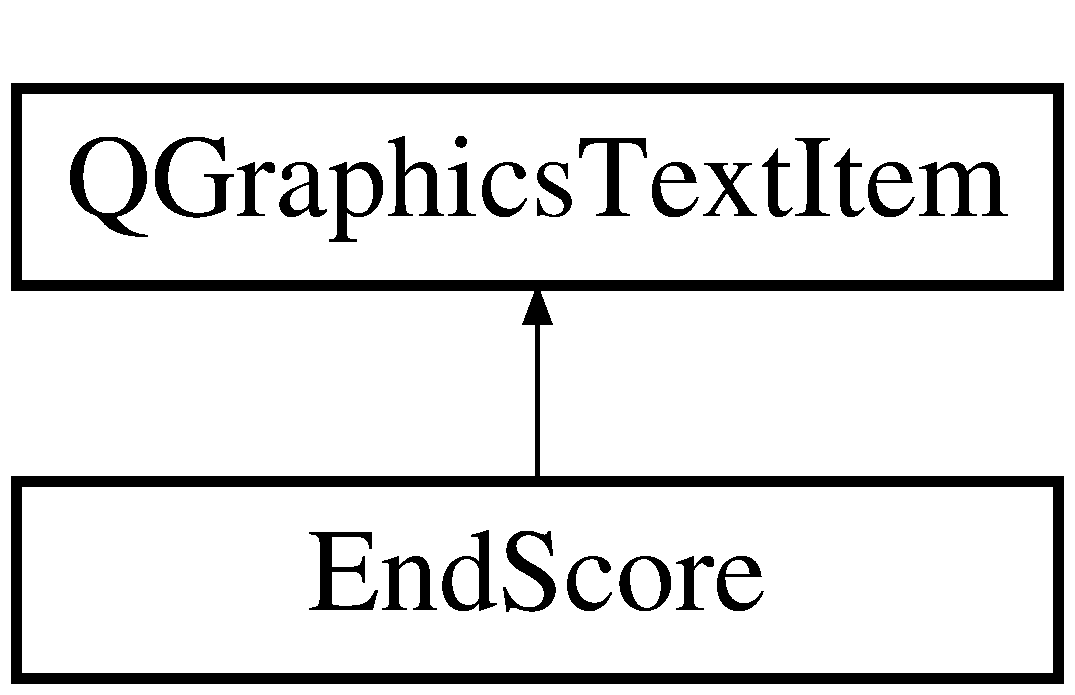
\includegraphics[height=2.000000cm]{classEndScore}
\end{center}
\end{figure}
\subsection*{Public Slots}
\begin{DoxyCompactItemize}
\item 
void {\bfseries add\+Amount} ()\hypertarget{classEndScore_aa7ceb6ad60b5a96265ac1343f21e2fa5}{}\label{classEndScore_aa7ceb6ad60b5a96265ac1343f21e2fa5}

\end{DoxyCompactItemize}
\subsection*{Public Member Functions}
\begin{DoxyCompactItemize}
\item 
{\bfseries End\+Score} (int input\+Score)\hypertarget{classEndScore_a5f7e9ff49366b9448242ba25b6dca5c2}{}\label{classEndScore_a5f7e9ff49366b9448242ba25b6dca5c2}

\end{DoxyCompactItemize}
\subsection*{Public Attributes}
\begin{DoxyCompactItemize}
\item 
int {\bfseries score}\hypertarget{classEndScore_abeb33879069b7d8352688b65af4c0382}{}\label{classEndScore_abeb33879069b7d8352688b65af4c0382}

\item 
int {\bfseries run}\hypertarget{classEndScore_a17bb38b597f93894e602d62851fc796c}{}\label{classEndScore_a17bb38b597f93894e602d62851fc796c}

\item 
Q\+Timer $\ast$ {\bfseries add\+Timer}\hypertarget{classEndScore_a88e820dfbf339eef4fe783661858bef1}{}\label{classEndScore_a88e820dfbf339eef4fe783661858bef1}

\end{DoxyCompactItemize}


The documentation for this class was generated from the following files\+:\begin{DoxyCompactItemize}
\item 
End\+Menu\+Scene/End\+Score.\+h\item 
End\+Menu\+Scene/End\+Score.\+cpp\end{DoxyCompactItemize}

\hypertarget{classGameEngine}{}\section{Game\+Engine Class Reference}
\label{classGameEngine}\index{Game\+Engine@{Game\+Engine}}
Inheritance diagram for Game\+Engine\+:\begin{figure}[H]
\begin{center}
\leavevmode
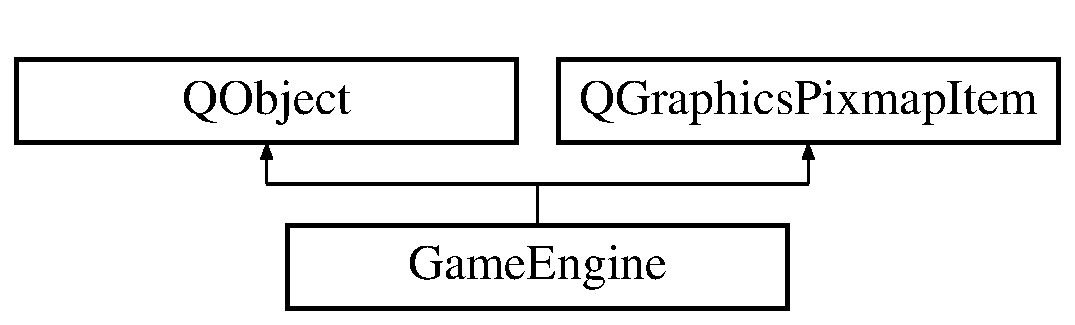
\includegraphics[height=2.000000cm]{classGameEngine}
\end{center}
\end{figure}
\subsection*{Signals}
\begin{DoxyCompactItemize}
\item 
void {\bfseries get\+Pull\+Pos} (int x, int y)\hypertarget{classGameEngine_a9c6f4ac73824ddc6b9ee9cbf0d3b8a42}{}\label{classGameEngine_a9c6f4ac73824ddc6b9ee9cbf0d3b8a42}

\item 
void {\bfseries release} ()\hypertarget{classGameEngine_aa4a838423f8055843a320b705ec80f59}{}\label{classGameEngine_aa4a838423f8055843a320b705ec80f59}

\item 
void {\bfseries use\+Special\+Ability} ()\hypertarget{classGameEngine_af35a3c4db56354360b88983d65b0c569}{}\label{classGameEngine_af35a3c4db56354360b88983d65b0c569}

\item 
void {\bfseries test\+End\+Game} ()\hypertarget{classGameEngine_a9072e3043080764b6ec831b598e42849}{}\label{classGameEngine_a9072e3043080764b6ec831b598e42849}

\end{DoxyCompactItemize}
\subsection*{Public Member Functions}
\begin{DoxyCompactItemize}
\item 
void {\bfseries key\+Press\+Event} (Q\+Key\+Event $\ast$event)\hypertarget{classGameEngine_aa73936c1c97161586f3293577e77f029}{}\label{classGameEngine_aa73936c1c97161586f3293577e77f029}

\item 
void {\bfseries key\+Release\+Event} (Q\+Key\+Event $\ast$event)\hypertarget{classGameEngine_a1cf0967d61ce05b59e0dcd3681cd3fdf}{}\label{classGameEngine_a1cf0967d61ce05b59e0dcd3681cd3fdf}

\item 
void {\bfseries mouse\+Press\+Event} (Q\+Graphics\+Scene\+Mouse\+Event $\ast$event)\hypertarget{classGameEngine_aea67b876a989ed7b7104bfac32fa17d4}{}\label{classGameEngine_aea67b876a989ed7b7104bfac32fa17d4}

\item 
void {\bfseries mouse\+Release\+Event} (Q\+Graphics\+Scene\+Mouse\+Event $\ast$event)\hypertarget{classGameEngine_afca8366e82ddb0299abc38caf8e627bf}{}\label{classGameEngine_afca8366e82ddb0299abc38caf8e627bf}

\item 
void {\bfseries mouse\+Move\+Event} (Q\+Graphics\+Scene\+Mouse\+Event $\ast$event)\hypertarget{classGameEngine_acb9e753f984d4f76d850a969844b499c}{}\label{classGameEngine_acb9e753f984d4f76d850a969844b499c}

\end{DoxyCompactItemize}


The documentation for this class was generated from the following files\+:\begin{DoxyCompactItemize}
\item 
Game\+Scene/Game\+Engine.\+h\item 
Game\+Scene/Game\+Engine.\+cpp\item 
moc\+\_\+\+Game\+Engine.\+cpp\end{DoxyCompactItemize}

\hypertarget{classGameItem}{}\section{Game\+Item Class Reference}
\label{classGameItem}\index{Game\+Item@{Game\+Item}}
Inheritance diagram for Game\+Item\+:\begin{figure}[H]
\begin{center}
\leavevmode
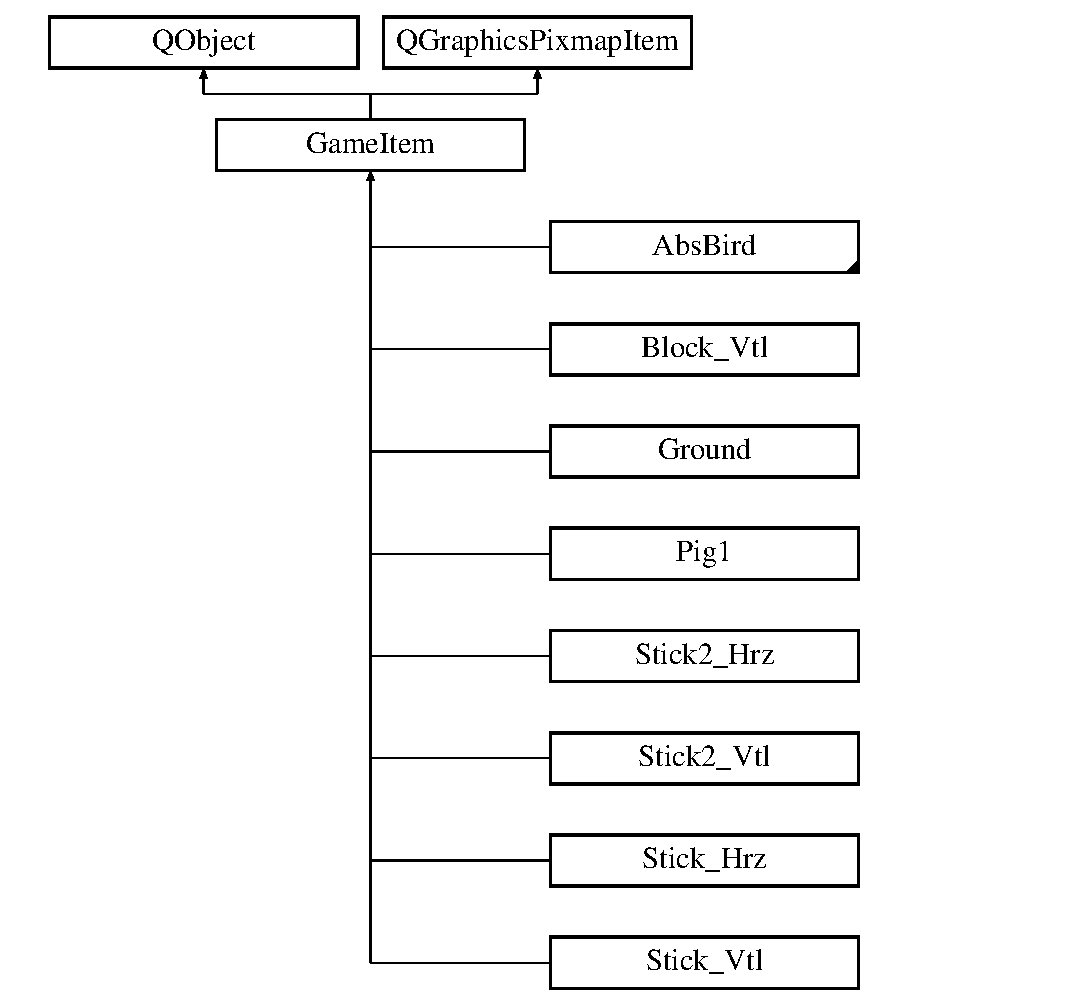
\includegraphics[height=10.000000cm]{classGameItem}
\end{center}
\end{figure}
\subsection*{Public Slots}
\begin{DoxyCompactItemize}
\item 
virtual void {\bfseries update\+Pos} ()\hypertarget{classGameItem_a9aadda5a28f03fc9976f8dd994ac2ce7}{}\label{classGameItem_a9aadda5a28f03fc9976f8dd994ac2ce7}

\end{DoxyCompactItemize}
\subsection*{Static Public Member Functions}
\begin{DoxyCompactItemize}
\item 
static float {\bfseries Pix\+To\+Meter\+\_\+x} (float Pix)\hypertarget{classGameItem_a58996071bc3039ae151f8a91024dcd17}{}\label{classGameItem_a58996071bc3039ae151f8a91024dcd17}

\item 
static float {\bfseries Meter\+To\+Pix\+\_\+x} (float Meter)\hypertarget{classGameItem_a4bc533807112f16030f646f32d587b7a}{}\label{classGameItem_a4bc533807112f16030f646f32d587b7a}

\item 
static float {\bfseries Pix\+To\+Meter\+\_\+y} (float Pix)\hypertarget{classGameItem_a5b2bcda53d0cebe338717347af7030cd}{}\label{classGameItem_a5b2bcda53d0cebe338717347af7030cd}

\item 
static float {\bfseries Meter\+To\+Pix\+\_\+y} (float Meter)\hypertarget{classGameItem_ac83bfc789dc61bf85cf0cce91a988116}{}\label{classGameItem_ac83bfc789dc61bf85cf0cce91a988116}

\item 
static float {\bfseries Rad\+To\+Deg} (float Rad)\hypertarget{classGameItem_a2d73b70119f56c82f53f92330fa99e0f}{}\label{classGameItem_a2d73b70119f56c82f53f92330fa99e0f}

\item 
static float {\bfseries Deg\+To\+Rad} (float Deg)\hypertarget{classGameItem_a229ae6c3829e1fa0fe25e172004042a3}{}\label{classGameItem_a229ae6c3829e1fa0fe25e172004042a3}

\end{DoxyCompactItemize}
\subsection*{Public Attributes}
\begin{DoxyCompactItemize}
\item 
string {\bfseries object\+Type}\hypertarget{classGameItem_a61814b6ad3ce20f5a8c69b43aa70379f}{}\label{classGameItem_a61814b6ad3ce20f5a8c69b43aa70379f}

\item 
\hyperlink{classItemData}{Item\+Data} $\ast$ {\bfseries item\+Data}\hypertarget{classGameItem_a00c0e196fe078eff9537af96827d9592}{}\label{classGameItem_a00c0e196fe078eff9537af96827d9592}

\item 
b2\+Body $\ast$ {\bfseries physic\+Body}\hypertarget{classGameItem_ac6324482db1a810a8aff077de71c9545}{}\label{classGameItem_ac6324482db1a810a8aff077de71c9545}

\item 
b2\+World $\ast$ {\bfseries in\+World}\hypertarget{classGameItem_a9c7ff677c89283296599f71d343cb607}{}\label{classGameItem_a9c7ff677c89283296599f71d343cb607}

\item 
b2\+Body\+Def $\ast$ {\bfseries body\+Struct}\hypertarget{classGameItem_a7a5131c14523447b600b7d4c65ded5b4}{}\label{classGameItem_a7a5131c14523447b600b7d4c65ded5b4}

\item 
b2\+Fixture\+Def $\ast$ {\bfseries body\+Fixture}\hypertarget{classGameItem_af20e53bedd210dd932493f21edbce5c0}{}\label{classGameItem_af20e53bedd210dd932493f21edbce5c0}

\item 
int {\bfseries health}\hypertarget{classGameItem_afa8d755b9557175edb2f4dc117900f3f}{}\label{classGameItem_afa8d755b9557175edb2f4dc117900f3f}

\end{DoxyCompactItemize}
\subsection*{Protected Member Functions}
\begin{DoxyCompactItemize}
\item 
void {\bfseries add\+Physics} ()\hypertarget{classGameItem_a22085b8c5a551d90d4132d0907b5439c}{}\label{classGameItem_a22085b8c5a551d90d4132d0907b5439c}

\end{DoxyCompactItemize}


The documentation for this class was generated from the following files\+:\begin{DoxyCompactItemize}
\item 
Game\+Scene/\+Abs\+Classes/Game\+Item.\+h\item 
Game\+Scene/\+Abs\+Classes/Game\+Item.\+cpp\end{DoxyCompactItemize}

\hypertarget{classGameScene}{}\section{Game\+Scene Class Reference}
\label{classGameScene}\index{Game\+Scene@{Game\+Scene}}
Inheritance diagram for Game\+Scene\+:\begin{figure}[H]
\begin{center}
\leavevmode
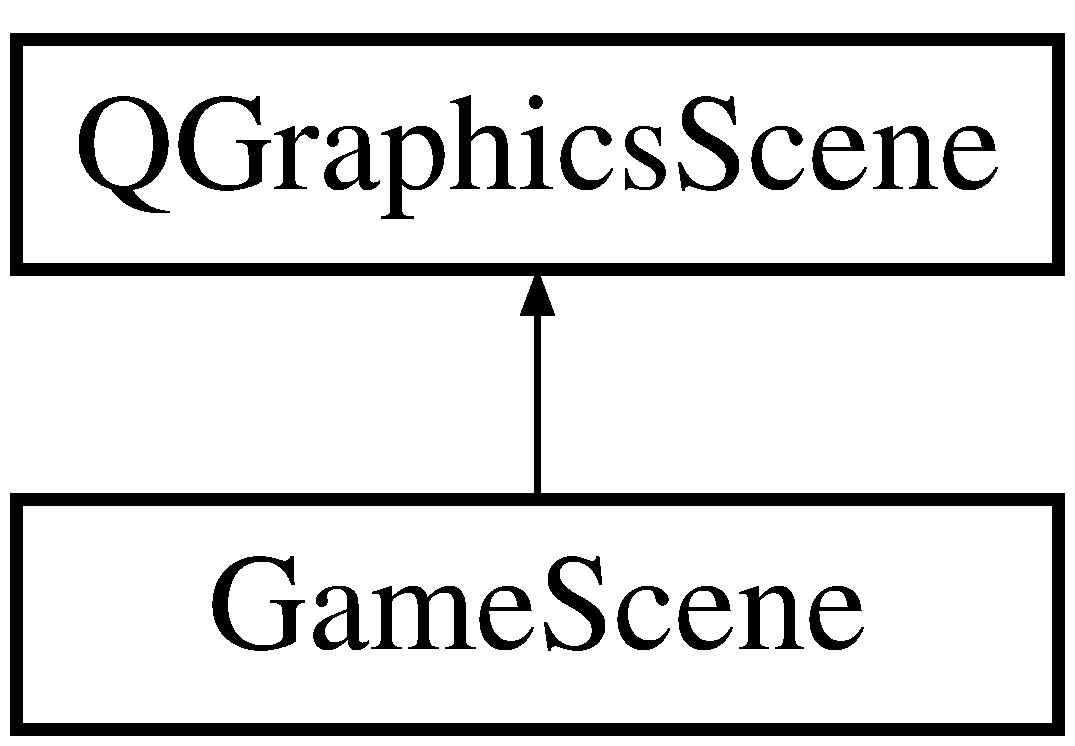
\includegraphics[height=2.000000cm]{classGameScene}
\end{center}
\end{figure}
\subsection*{Public Slots}
\begin{DoxyCompactItemize}
\item 
void {\bfseries update\+World} ()\hypertarget{classGameScene_a3cd26f3187b16c051adfc3d793a779fe}{}\label{classGameScene_a3cd26f3187b16c051adfc3d793a779fe}

\item 
void {\bfseries release\+Bird} ()\hypertarget{classGameScene_a8f3287bb12c938b3136277ee4a85535a}{}\label{classGameScene_a8f3287bb12c938b3136277ee4a85535a}

\item 
void {\bfseries set\+New\+Bird} ()\hypertarget{classGameScene_a37a1d18f300ea8d1c2cd8f317b3494e4}{}\label{classGameScene_a37a1d18f300ea8d1c2cd8f317b3494e4}

\item 
void {\bfseries use\+Special\+Ability} ()\hypertarget{classGameScene_afd5205ce0002a5ede28191c85ac2609c}{}\label{classGameScene_afd5205ce0002a5ede28191c85ac2609c}

\item 
void {\bfseries spawn\+Blue\+Child} (int x, int y)\hypertarget{classGameScene_a8c227f4c754e4ecaf5ffeee55cd5cf3d}{}\label{classGameScene_a8c227f4c754e4ecaf5ffeee55cd5cf3d}

\item 
void {\bfseries delete\+Pig} ()\hypertarget{classGameScene_afb7e34be8e0924d8a201533a85953772}{}\label{classGameScene_afb7e34be8e0924d8a201533a85953772}

\item 
void {\bfseries test\+End\+Game} ()\hypertarget{classGameScene_a00aec73ec8bce50ec8901dd56e32d0a5}{}\label{classGameScene_a00aec73ec8bce50ec8901dd56e32d0a5}

\end{DoxyCompactItemize}
\subsection*{Signals}
\begin{DoxyCompactItemize}
\item 
void {\bfseries set\+End\+Scene} (int, int)\hypertarget{classGameScene_a134cbab1d01f474d1899d2d4b35fe16c}{}\label{classGameScene_a134cbab1d01f474d1899d2d4b35fe16c}

\end{DoxyCompactItemize}
\subsection*{Public Member Functions}
\begin{DoxyCompactItemize}
\item 
void {\bfseries setup\+Stage} ()\hypertarget{classGameScene_a9de3918bb8c2b241bc67a260e7c579af}{}\label{classGameScene_a9de3918bb8c2b241bc67a260e7c579af}

\end{DoxyCompactItemize}
\subsection*{Public Attributes}
\begin{DoxyCompactItemize}
\item 
Q\+Timer $\ast$ {\bfseries timer60}\hypertarget{classGameScene_af6fc4df0ed326e09aa974df571c22288}{}\label{classGameScene_af6fc4df0ed326e09aa974df571c22288}

\item 
\hyperlink{classGameEngine}{Game\+Engine} $\ast$ {\bfseries game\+Engine}\hypertarget{classGameScene_a129381cd74fb68cfaeccd96a5ecc4ad7}{}\label{classGameScene_a129381cd74fb68cfaeccd96a5ecc4ad7}

\end{DoxyCompactItemize}


The documentation for this class was generated from the following files\+:\begin{DoxyCompactItemize}
\item 
Game\+Scene/Game\+Scene.\+h\item 
Game\+Scene/Game\+Scene.\+cpp\item 
moc\+\_\+\+Game\+Scene.\+cpp\end{DoxyCompactItemize}

\hypertarget{classGameView}{}\section{Game\+View Class Reference}
\label{classGameView}\index{Game\+View@{Game\+View}}
Inheritance diagram for Game\+View\+:\begin{figure}[H]
\begin{center}
\leavevmode
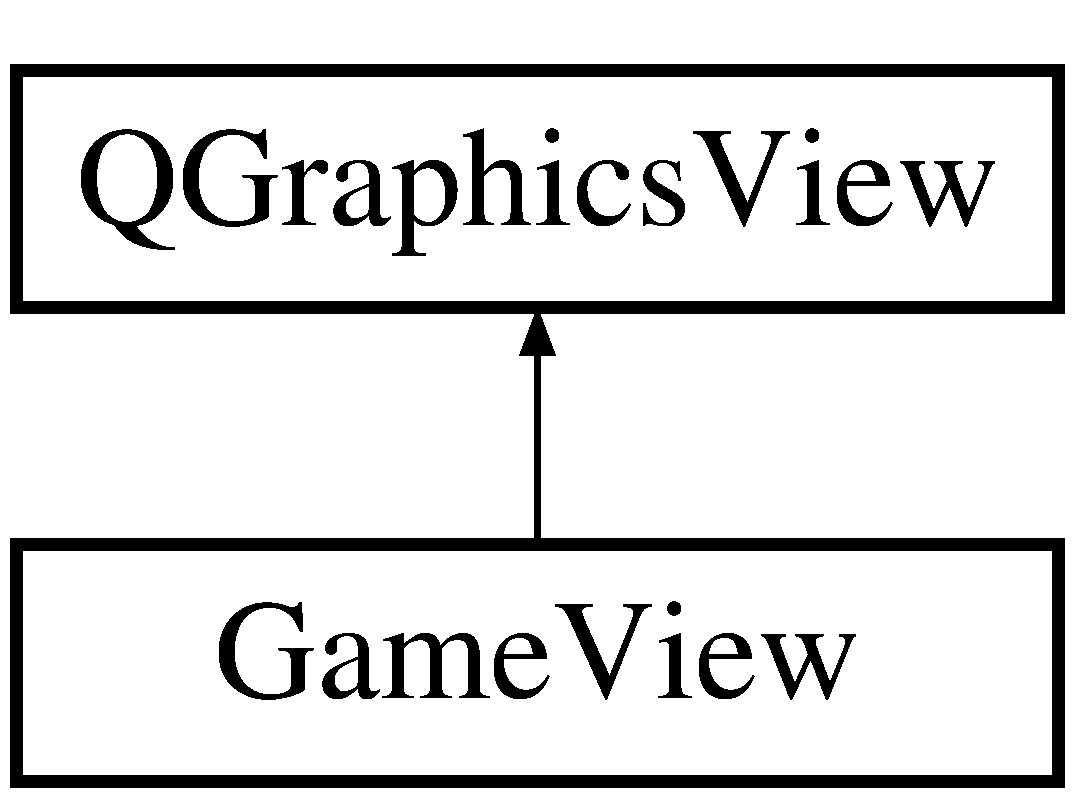
\includegraphics[height=2.000000cm]{classGameView}
\end{center}
\end{figure}
\subsection*{Public Slots}
\begin{DoxyCompactItemize}
\item 
void {\bfseries set\+End\+Game\+Scene} (int score\+Get, int bird\+Used)\hypertarget{classGameView_a90b6c5b6b154f1c455ab03522b866fda}{}\label{classGameView_a90b6c5b6b154f1c455ab03522b866fda}

\item 
void {\bfseries set\+Play\+Again} ()\hypertarget{classGameView_a904299204c154220c8051340845eec99}{}\label{classGameView_a904299204c154220c8051340845eec99}

\item 
void {\bfseries exit\+Game} ()\hypertarget{classGameView_aeb490f4e448fac7f2eb24fb39f8227d4}{}\label{classGameView_aeb490f4e448fac7f2eb24fb39f8227d4}

\end{DoxyCompactItemize}
\subsection*{Signals}
\begin{DoxyCompactItemize}
\item 
void {\bfseries quit\+Game} ()\hypertarget{classGameView_a91360001693a1fe1d2a610d7f14a2876}{}\label{classGameView_a91360001693a1fe1d2a610d7f14a2876}

\end{DoxyCompactItemize}
\subsection*{Public Member Functions}
\begin{DoxyCompactItemize}
\item 
{\bfseries Game\+View} (Q\+Widget $\ast$parent=0)\hypertarget{classGameView_a6f41d09f51d2abd6abb3b99e5da8ef6f}{}\label{classGameView_a6f41d09f51d2abd6abb3b99e5da8ef6f}

\end{DoxyCompactItemize}
\subsection*{Public Attributes}
\begin{DoxyCompactItemize}
\item 
\hyperlink{classGameScene}{Game\+Scene} $\ast$ {\bfseries game\+Scene}\hypertarget{classGameView_a7c4d2d02b91a7313d4fcfe3419eb3feb}{}\label{classGameView_a7c4d2d02b91a7313d4fcfe3419eb3feb}

\item 
\hyperlink{classEndMenuScene}{End\+Menu\+Scene} $\ast$ {\bfseries end\+Menu\+Scene}\hypertarget{classGameView_ade77636f2cd8eeb6d1bb49b524df06bb}{}\label{classGameView_ade77636f2cd8eeb6d1bb49b524df06bb}

\end{DoxyCompactItemize}


The documentation for this class was generated from the following files\+:\begin{DoxyCompactItemize}
\item 
Game\+View.\+h\item 
Game\+View.\+cpp\item 
moc\+\_\+\+Game\+View.\+cpp\end{DoxyCompactItemize}

\hypertarget{classGround}{}\section{Ground Class Reference}
\label{classGround}\index{Ground@{Ground}}
Inheritance diagram for Ground\+:\begin{figure}[H]
\begin{center}
\leavevmode
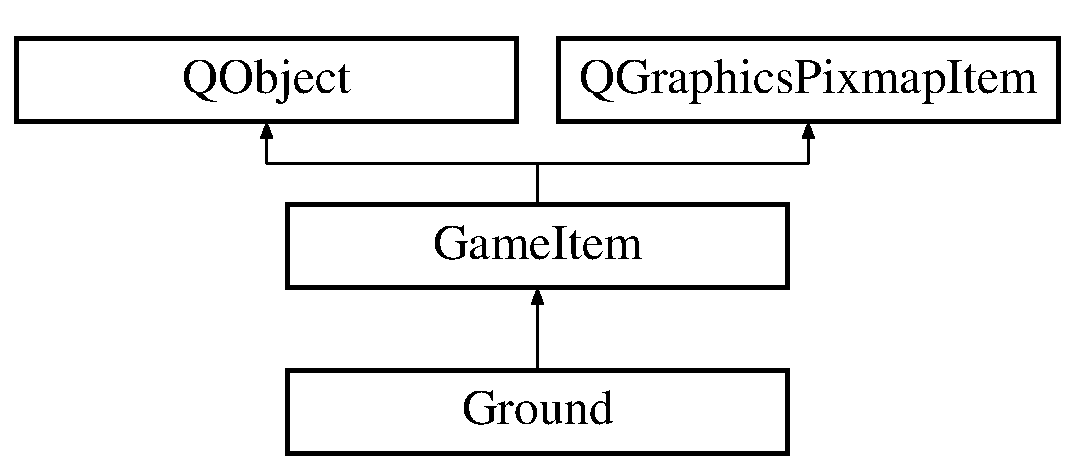
\includegraphics[height=3.000000cm]{classGround}
\end{center}
\end{figure}
\subsection*{Public Member Functions}
\begin{DoxyCompactItemize}
\item 
{\bfseries Ground} (b2\+World $\ast$input\+World)\hypertarget{classGround_ae19f2ed3cb333e1f6e2c03aa76a8726d}{}\label{classGround_ae19f2ed3cb333e1f6e2c03aa76a8726d}

\end{DoxyCompactItemize}
\subsection*{Additional Inherited Members}


The documentation for this class was generated from the following files\+:\begin{DoxyCompactItemize}
\item 
Game\+Scene/\+Random\+Items/Ground.\+h\item 
Game\+Scene/\+Random\+Items/Ground.\+cpp\end{DoxyCompactItemize}

\hypertarget{classItemData}{}\section{Item\+Data Class Reference}
\label{classItemData}\index{Item\+Data@{Item\+Data}}
\subsection*{Public Attributes}
\begin{DoxyCompactItemize}
\item 
string {\bfseries object\+Type}\hypertarget{classItemData_a43c5389381a9741d73e32549129500dc}{}\label{classItemData_a43c5389381a9741d73e32549129500dc}

\item 
void $\ast$ {\bfseries scene\+Object}\hypertarget{classItemData_ab352e8ff54f381c67c6d9d9fff6f1671}{}\label{classItemData_ab352e8ff54f381c67c6d9d9fff6f1671}

\item 
void $\ast$ {\bfseries body\+Object}\hypertarget{classItemData_a2d72daf62224350e9022479954195fe8}{}\label{classItemData_a2d72daf62224350e9022479954195fe8}

\end{DoxyCompactItemize}


The documentation for this class was generated from the following files\+:\begin{DoxyCompactItemize}
\item 
Game\+Scene/\+Abs\+Classes/Item\+Data.\+h\item 
Game\+Scene/\+Abs\+Classes/Item\+Data.\+cpp\end{DoxyCompactItemize}

\hypertarget{classLeaveButton}{}\section{Leave\+Button Class Reference}
\label{classLeaveButton}\index{Leave\+Button@{Leave\+Button}}
Inheritance diagram for Leave\+Button\+:\begin{figure}[H]
\begin{center}
\leavevmode
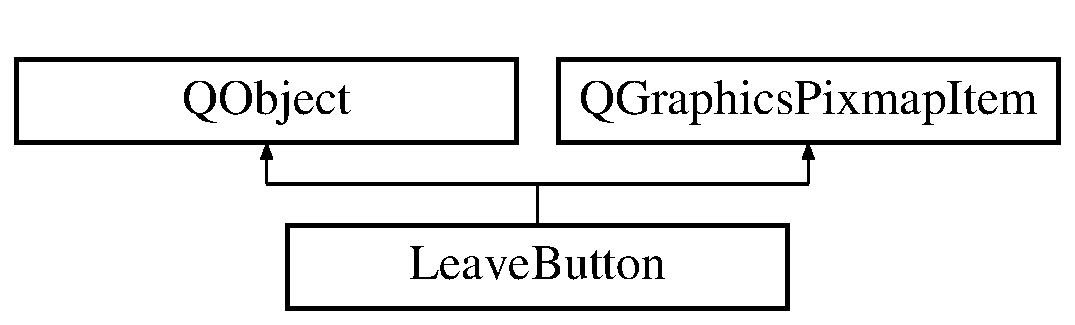
\includegraphics[height=2.000000cm]{classLeaveButton}
\end{center}
\end{figure}
\subsection*{Signals}
\begin{DoxyCompactItemize}
\item 
void {\bfseries clicked} ()\hypertarget{classLeaveButton_a23c0fdc8ebbe3f2ce2a817e3587d634d}{}\label{classLeaveButton_a23c0fdc8ebbe3f2ce2a817e3587d634d}

\end{DoxyCompactItemize}
\subsection*{Public Member Functions}
\begin{DoxyCompactItemize}
\item 
void {\bfseries mouse\+Press\+Event} (Q\+Graphics\+Scene\+Mouse\+Event $\ast$event)\hypertarget{classLeaveButton_ae627a5bbcd17ae533b10efc57d80afe6}{}\label{classLeaveButton_ae627a5bbcd17ae533b10efc57d80afe6}

\item 
void {\bfseries hover\+Enter\+Event} (Q\+Graphics\+Scene\+Hover\+Event $\ast$event)\hypertarget{classLeaveButton_a7e3b2d000b0630daa8366e547a06e059}{}\label{classLeaveButton_a7e3b2d000b0630daa8366e547a06e059}

\item 
void {\bfseries hover\+Leave\+Event} (Q\+Graphics\+Scene\+Hover\+Event $\ast$event)\hypertarget{classLeaveButton_a709352208ac9bed883c40e417e4c13dd}{}\label{classLeaveButton_a709352208ac9bed883c40e417e4c13dd}

\end{DoxyCompactItemize}


The documentation for this class was generated from the following files\+:\begin{DoxyCompactItemize}
\item 
End\+Menu\+Scene/Leave\+Button.\+h\item 
End\+Menu\+Scene/Leave\+Button.\+cpp\item 
moc\+\_\+\+Leave\+Button.\+cpp\end{DoxyCompactItemize}

\hypertarget{classMainWindow}{}\section{Main\+Window Class Reference}
\label{classMainWindow}\index{Main\+Window@{Main\+Window}}
Inheritance diagram for Main\+Window\+:\begin{figure}[H]
\begin{center}
\leavevmode
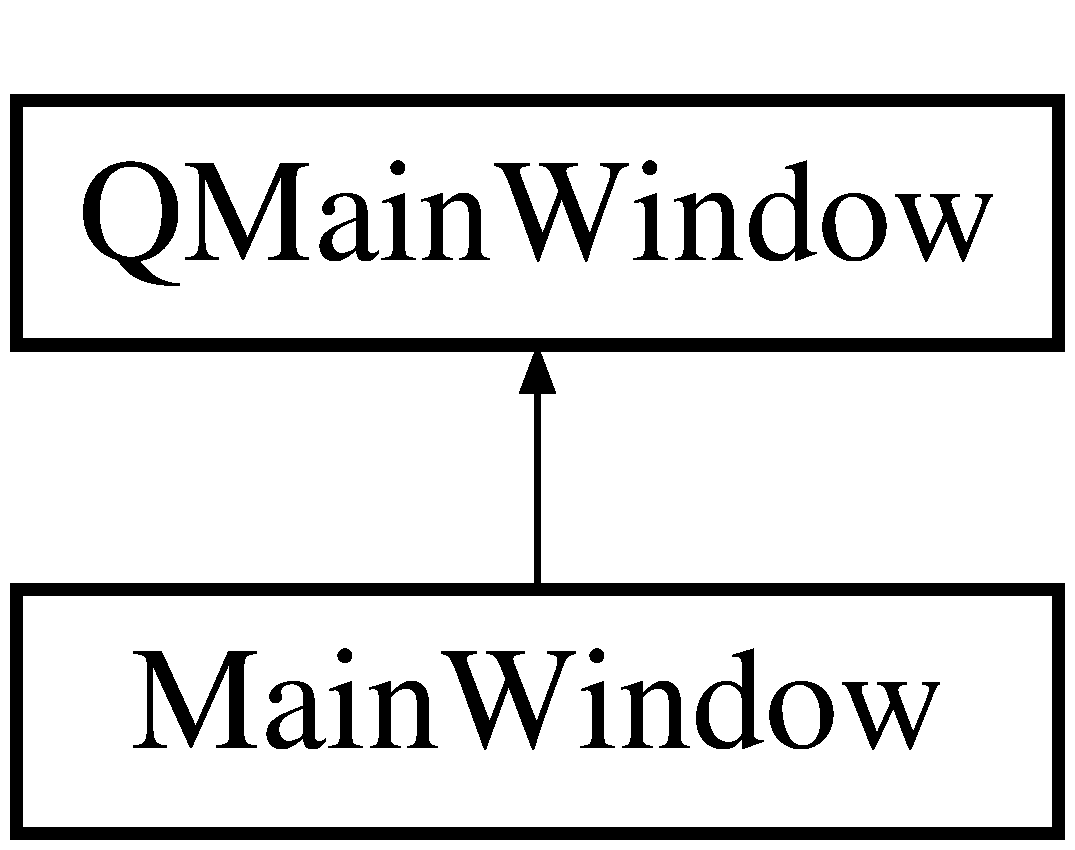
\includegraphics[height=2.000000cm]{classMainWindow}
\end{center}
\end{figure}
\subsection*{Public Member Functions}
\begin{DoxyCompactItemize}
\item 
{\bfseries Main\+Window} (Q\+Widget $\ast$parent=0)\hypertarget{classMainWindow_a8b244be8b7b7db1b08de2a2acb9409db}{}\label{classMainWindow_a8b244be8b7b7db1b08de2a2acb9409db}

\end{DoxyCompactItemize}


The documentation for this class was generated from the following files\+:\begin{DoxyCompactItemize}
\item 
Main\+Window.\+h\item 
Main\+Window.\+cpp\end{DoxyCompactItemize}

\hypertarget{classPig1}{}\section{Pig1 Class Reference}
\label{classPig1}\index{Pig1@{Pig1}}
Inheritance diagram for Pig1\+:\begin{figure}[H]
\begin{center}
\leavevmode
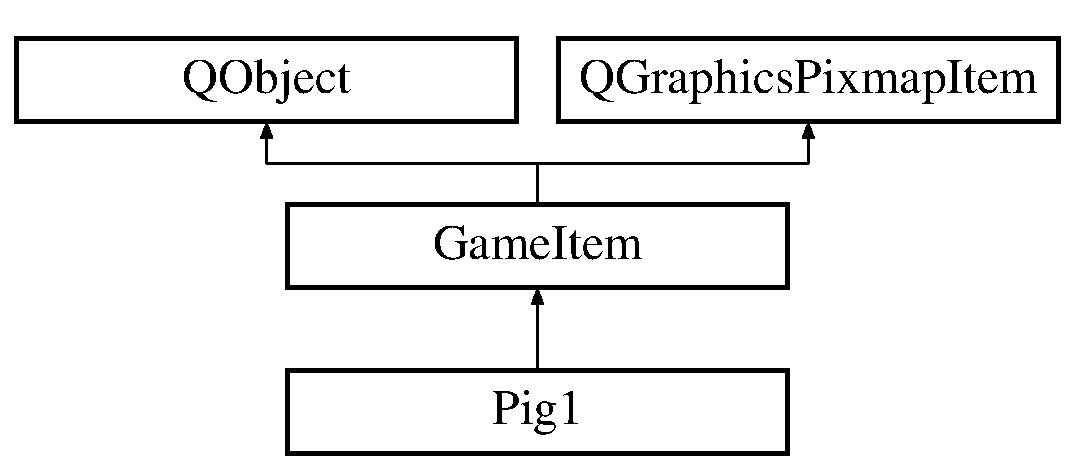
\includegraphics[height=3.000000cm]{classPig1}
\end{center}
\end{figure}
\subsection*{Public Slots}
\begin{DoxyCompactItemize}
\item 
void {\bfseries update\+Pos} ()\hypertarget{classPig1_a64bbc503af0ba01b038099f5d16e978a}{}\label{classPig1_a64bbc503af0ba01b038099f5d16e978a}

\end{DoxyCompactItemize}
\subsection*{Public Member Functions}
\begin{DoxyCompactItemize}
\item 
{\bfseries Pig1} (b2\+World $\ast$input\+World, int inputX, int inputY)\hypertarget{classPig1_a31f8ee0c55f6ccd6714029f83f62dc6d}{}\label{classPig1_a31f8ee0c55f6ccd6714029f83f62dc6d}

\end{DoxyCompactItemize}
\subsection*{Additional Inherited Members}


The documentation for this class was generated from the following files\+:\begin{DoxyCompactItemize}
\item 
Game\+Scene/\+Pigs/Pig1.\+h\item 
Game\+Scene/\+Pigs/Pig1.\+cpp\end{DoxyCompactItemize}

\hypertarget{classPlayScore}{}\section{Play\+Score Class Reference}
\label{classPlayScore}\index{Play\+Score@{Play\+Score}}
Inheritance diagram for Play\+Score\+:\begin{figure}[H]
\begin{center}
\leavevmode
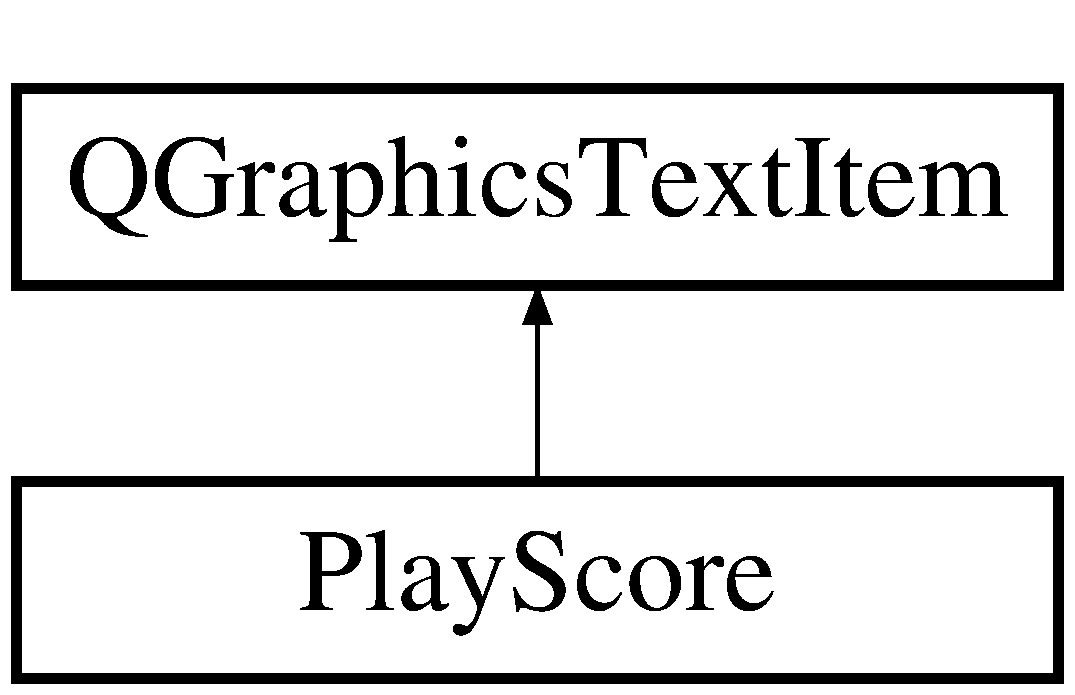
\includegraphics[height=2.000000cm]{classPlayScore}
\end{center}
\end{figure}
\subsection*{Public Slots}
\begin{DoxyCompactItemize}
\item 
void {\bfseries add\+Score} (int amount)\hypertarget{classPlayScore_a9f72ef9c1592287a2a9ccab6e0692612}{}\label{classPlayScore_a9f72ef9c1592287a2a9ccab6e0692612}

\end{DoxyCompactItemize}
\subsection*{Public Attributes}
\begin{DoxyCompactItemize}
\item 
int {\bfseries score}\hypertarget{classPlayScore_a1f561d7ce7d52b44c72694489444ad8a}{}\label{classPlayScore_a1f561d7ce7d52b44c72694489444ad8a}

\end{DoxyCompactItemize}


The documentation for this class was generated from the following files\+:\begin{DoxyCompactItemize}
\item 
Game\+Scene/Play\+Score.\+h\item 
Game\+Scene/Play\+Score.\+cpp\end{DoxyCompactItemize}

\hypertarget{structqt__meta__stringdata__AbsBird__t}{}\section{qt\+\_\+meta\+\_\+stringdata\+\_\+\+Abs\+Bird\+\_\+t Struct Reference}
\label{structqt__meta__stringdata__AbsBird__t}\index{qt\+\_\+meta\+\_\+stringdata\+\_\+\+Abs\+Bird\+\_\+t@{qt\+\_\+meta\+\_\+stringdata\+\_\+\+Abs\+Bird\+\_\+t}}
\subsection*{Public Attributes}
\begin{DoxyCompactItemize}
\item 
Q\+Byte\+Array\+Data {\bfseries data} \mbox{[}10\mbox{]}\hypertarget{structqt__meta__stringdata__AbsBird__t_ab292b9f61d163bc9a44fe38ac593e1a9}{}\label{structqt__meta__stringdata__AbsBird__t_ab292b9f61d163bc9a44fe38ac593e1a9}

\item 
char {\bfseries stringdata0} \mbox{[}75\mbox{]}\hypertarget{structqt__meta__stringdata__AbsBird__t_a6ad291a8804cc2be83dd2897537b708d}{}\label{structqt__meta__stringdata__AbsBird__t_a6ad291a8804cc2be83dd2897537b708d}

\end{DoxyCompactItemize}


The documentation for this struct was generated from the following file\+:\begin{DoxyCompactItemize}
\item 
moc\+\_\+\+Abs\+Bird.\+cpp\end{DoxyCompactItemize}

\hypertarget{structqt__meta__stringdata__BigBird__t}{}\section{qt\+\_\+meta\+\_\+stringdata\+\_\+\+Big\+Bird\+\_\+t Struct Reference}
\label{structqt__meta__stringdata__BigBird__t}\index{qt\+\_\+meta\+\_\+stringdata\+\_\+\+Big\+Bird\+\_\+t@{qt\+\_\+meta\+\_\+stringdata\+\_\+\+Big\+Bird\+\_\+t}}
\subsection*{Public Attributes}
\begin{DoxyCompactItemize}
\item 
Q\+Byte\+Array\+Data {\bfseries data} \mbox{[}7\mbox{]}\hypertarget{structqt__meta__stringdata__BigBird__t_a56b48e472c3510a7b32b2d878545ae3b}{}\label{structqt__meta__stringdata__BigBird__t_a56b48e472c3510a7b32b2d878545ae3b}

\item 
char {\bfseries stringdata0} \mbox{[}49\mbox{]}\hypertarget{structqt__meta__stringdata__BigBird__t_aa4f91a78b5eff353d11d9612c2b169cd}{}\label{structqt__meta__stringdata__BigBird__t_aa4f91a78b5eff353d11d9612c2b169cd}

\end{DoxyCompactItemize}


The documentation for this struct was generated from the following file\+:\begin{DoxyCompactItemize}
\item 
moc\+\_\+\+Big\+Bird.\+cpp\end{DoxyCompactItemize}

\hypertarget{structqt__meta__stringdata__BirdUsedAmount__t}{}\section{qt\+\_\+meta\+\_\+stringdata\+\_\+\+Bird\+Used\+Amount\+\_\+t Struct Reference}
\label{structqt__meta__stringdata__BirdUsedAmount__t}\index{qt\+\_\+meta\+\_\+stringdata\+\_\+\+Bird\+Used\+Amount\+\_\+t@{qt\+\_\+meta\+\_\+stringdata\+\_\+\+Bird\+Used\+Amount\+\_\+t}}
\subsection*{Public Attributes}
\begin{DoxyCompactItemize}
\item 
Q\+Byte\+Array\+Data {\bfseries data} \mbox{[}3\mbox{]}\hypertarget{structqt__meta__stringdata__BirdUsedAmount__t_a420170ebae5a2ea1aa5444671bcc9eee}{}\label{structqt__meta__stringdata__BirdUsedAmount__t_a420170ebae5a2ea1aa5444671bcc9eee}

\item 
char {\bfseries stringdata0} \mbox{[}26\mbox{]}\hypertarget{structqt__meta__stringdata__BirdUsedAmount__t_ab49930d2238024145b2ab31abe5d9b02}{}\label{structqt__meta__stringdata__BirdUsedAmount__t_ab49930d2238024145b2ab31abe5d9b02}

\end{DoxyCompactItemize}


The documentation for this struct was generated from the following file\+:\begin{DoxyCompactItemize}
\item 
moc\+\_\+\+Bird\+Used\+Amount.\+cpp\end{DoxyCompactItemize}

\hypertarget{structqt__meta__stringdata__Block__Vtl__t}{}\section{qt\+\_\+meta\+\_\+stringdata\+\_\+\+Block\+\_\+\+Vtl\+\_\+t Struct Reference}
\label{structqt__meta__stringdata__Block__Vtl__t}\index{qt\+\_\+meta\+\_\+stringdata\+\_\+\+Block\+\_\+\+Vtl\+\_\+t@{qt\+\_\+meta\+\_\+stringdata\+\_\+\+Block\+\_\+\+Vtl\+\_\+t}}
\subsection*{Public Attributes}
\begin{DoxyCompactItemize}
\item 
Q\+Byte\+Array\+Data {\bfseries data} \mbox{[}1\mbox{]}\hypertarget{structqt__meta__stringdata__Block__Vtl__t_a62b56a8930213f2c3931ce3cf1929261}{}\label{structqt__meta__stringdata__Block__Vtl__t_a62b56a8930213f2c3931ce3cf1929261}

\item 
char {\bfseries stringdata0} \mbox{[}10\mbox{]}\hypertarget{structqt__meta__stringdata__Block__Vtl__t_a60c5abdd7ce66a74654084ba3855c32c}{}\label{structqt__meta__stringdata__Block__Vtl__t_a60c5abdd7ce66a74654084ba3855c32c}

\end{DoxyCompactItemize}


The documentation for this struct was generated from the following file\+:\begin{DoxyCompactItemize}
\item 
moc\+\_\+\+Block\+\_\+\+Vtl.\+cpp\end{DoxyCompactItemize}

\hypertarget{structqt__meta__stringdata__BlueBird__t}{}\section{qt\+\_\+meta\+\_\+stringdata\+\_\+\+Blue\+Bird\+\_\+t Struct Reference}
\label{structqt__meta__stringdata__BlueBird__t}\index{qt\+\_\+meta\+\_\+stringdata\+\_\+\+Blue\+Bird\+\_\+t@{qt\+\_\+meta\+\_\+stringdata\+\_\+\+Blue\+Bird\+\_\+t}}
\subsection*{Public Attributes}
\begin{DoxyCompactItemize}
\item 
Q\+Byte\+Array\+Data {\bfseries data} \mbox{[}7\mbox{]}\hypertarget{structqt__meta__stringdata__BlueBird__t_aaaf00ed7b3c9a686945dab8de652d386}{}\label{structqt__meta__stringdata__BlueBird__t_aaaf00ed7b3c9a686945dab8de652d386}

\item 
char {\bfseries stringdata0} \mbox{[}54\mbox{]}\hypertarget{structqt__meta__stringdata__BlueBird__t_aa9cc3b163d67256197fcadfa69aa6575}{}\label{structqt__meta__stringdata__BlueBird__t_aa9cc3b163d67256197fcadfa69aa6575}

\end{DoxyCompactItemize}


The documentation for this struct was generated from the following file\+:\begin{DoxyCompactItemize}
\item 
moc\+\_\+\+Blue\+Bird.\+cpp\end{DoxyCompactItemize}

\hypertarget{structqt__meta__stringdata__CollisionListener__t}{}\section{qt\+\_\+meta\+\_\+stringdata\+\_\+\+Collision\+Listener\+\_\+t Struct Reference}
\label{structqt__meta__stringdata__CollisionListener__t}\index{qt\+\_\+meta\+\_\+stringdata\+\_\+\+Collision\+Listener\+\_\+t@{qt\+\_\+meta\+\_\+stringdata\+\_\+\+Collision\+Listener\+\_\+t}}
\subsection*{Public Attributes}
\begin{DoxyCompactItemize}
\item 
Q\+Byte\+Array\+Data {\bfseries data} \mbox{[}4\mbox{]}\hypertarget{structqt__meta__stringdata__CollisionListener__t_a2fc55762bb9073c96f6b08b7bd892d05}{}\label{structqt__meta__stringdata__CollisionListener__t_a2fc55762bb9073c96f6b08b7bd892d05}

\item 
char {\bfseries stringdata0} \mbox{[}38\mbox{]}\hypertarget{structqt__meta__stringdata__CollisionListener__t_a87776e0ada4783e0e941a8b8282d41f0}{}\label{structqt__meta__stringdata__CollisionListener__t_a87776e0ada4783e0e941a8b8282d41f0}

\end{DoxyCompactItemize}


The documentation for this struct was generated from the following file\+:\begin{DoxyCompactItemize}
\item 
moc\+\_\+\+Collision\+Listener.\+cpp\end{DoxyCompactItemize}

\hypertarget{structqt__meta__stringdata__EndScore__t}{}\section{qt\+\_\+meta\+\_\+stringdata\+\_\+\+End\+Score\+\_\+t Struct Reference}
\label{structqt__meta__stringdata__EndScore__t}\index{qt\+\_\+meta\+\_\+stringdata\+\_\+\+End\+Score\+\_\+t@{qt\+\_\+meta\+\_\+stringdata\+\_\+\+End\+Score\+\_\+t}}
\subsection*{Public Attributes}
\begin{DoxyCompactItemize}
\item 
Q\+Byte\+Array\+Data {\bfseries data} \mbox{[}3\mbox{]}\hypertarget{structqt__meta__stringdata__EndScore__t_a9f80171958b2e7040252027cdf76b0ae}{}\label{structqt__meta__stringdata__EndScore__t_a9f80171958b2e7040252027cdf76b0ae}

\item 
char {\bfseries stringdata0} \mbox{[}20\mbox{]}\hypertarget{structqt__meta__stringdata__EndScore__t_a686bc2f2054d669307663e769f68dae2}{}\label{structqt__meta__stringdata__EndScore__t_a686bc2f2054d669307663e769f68dae2}

\end{DoxyCompactItemize}


The documentation for this struct was generated from the following file\+:\begin{DoxyCompactItemize}
\item 
moc\+\_\+\+End\+Score.\+cpp\end{DoxyCompactItemize}

\hypertarget{structqt__meta__stringdata__GameEngine__t}{}\section{qt\+\_\+meta\+\_\+stringdata\+\_\+\+Game\+Engine\+\_\+t Struct Reference}
\label{structqt__meta__stringdata__GameEngine__t}\index{qt\+\_\+meta\+\_\+stringdata\+\_\+\+Game\+Engine\+\_\+t@{qt\+\_\+meta\+\_\+stringdata\+\_\+\+Game\+Engine\+\_\+t}}
\subsection*{Public Attributes}
\begin{DoxyCompactItemize}
\item 
Q\+Byte\+Array\+Data {\bfseries data} \mbox{[}8\mbox{]}\hypertarget{structqt__meta__stringdata__GameEngine__t_a011ffd9cd6cbbd9539314be8c9786d27}{}\label{structqt__meta__stringdata__GameEngine__t_a011ffd9cd6cbbd9539314be8c9786d27}

\item 
char {\bfseries stringdata0} \mbox{[}65\mbox{]}\hypertarget{structqt__meta__stringdata__GameEngine__t_a4fcab7fae1a0dff7923e0662d1b906a7}{}\label{structqt__meta__stringdata__GameEngine__t_a4fcab7fae1a0dff7923e0662d1b906a7}

\end{DoxyCompactItemize}


The documentation for this struct was generated from the following file\+:\begin{DoxyCompactItemize}
\item 
moc\+\_\+\+Game\+Engine.\+cpp\end{DoxyCompactItemize}

\hypertarget{structqt__meta__stringdata__GameItem__t}{}\section{qt\+\_\+meta\+\_\+stringdata\+\_\+\+Game\+Item\+\_\+t Struct Reference}
\label{structqt__meta__stringdata__GameItem__t}\index{qt\+\_\+meta\+\_\+stringdata\+\_\+\+Game\+Item\+\_\+t@{qt\+\_\+meta\+\_\+stringdata\+\_\+\+Game\+Item\+\_\+t}}
\subsection*{Public Attributes}
\begin{DoxyCompactItemize}
\item 
Q\+Byte\+Array\+Data {\bfseries data} \mbox{[}3\mbox{]}\hypertarget{structqt__meta__stringdata__GameItem__t_a6d899d168e51660ea57dd55d93245086}{}\label{structqt__meta__stringdata__GameItem__t_a6d899d168e51660ea57dd55d93245086}

\item 
char {\bfseries stringdata0} \mbox{[}20\mbox{]}\hypertarget{structqt__meta__stringdata__GameItem__t_a5b537ade13ffa2d4c9c96082f4d60d2c}{}\label{structqt__meta__stringdata__GameItem__t_a5b537ade13ffa2d4c9c96082f4d60d2c}

\end{DoxyCompactItemize}


The documentation for this struct was generated from the following file\+:\begin{DoxyCompactItemize}
\item 
moc\+\_\+\+Game\+Item.\+cpp\end{DoxyCompactItemize}

\hypertarget{structqt__meta__stringdata__GameScene__t}{}\section{qt\+\_\+meta\+\_\+stringdata\+\_\+\+Game\+Scene\+\_\+t Struct Reference}
\label{structqt__meta__stringdata__GameScene__t}\index{qt\+\_\+meta\+\_\+stringdata\+\_\+\+Game\+Scene\+\_\+t@{qt\+\_\+meta\+\_\+stringdata\+\_\+\+Game\+Scene\+\_\+t}}
\subsection*{Public Attributes}
\begin{DoxyCompactItemize}
\item 
Q\+Byte\+Array\+Data {\bfseries data} \mbox{[}12\mbox{]}\hypertarget{structqt__meta__stringdata__GameScene__t_a26503bb9519f5b841771365ea207a341}{}\label{structqt__meta__stringdata__GameScene__t_a26503bb9519f5b841771365ea207a341}

\item 
char {\bfseries stringdata0} \mbox{[}117\mbox{]}\hypertarget{structqt__meta__stringdata__GameScene__t_a922115ecfeb72b9395decb6d07c2a4fd}{}\label{structqt__meta__stringdata__GameScene__t_a922115ecfeb72b9395decb6d07c2a4fd}

\end{DoxyCompactItemize}


The documentation for this struct was generated from the following file\+:\begin{DoxyCompactItemize}
\item 
moc\+\_\+\+Game\+Scene.\+cpp\end{DoxyCompactItemize}

\hypertarget{structqt__meta__stringdata__GameView__t}{}\section{qt\+\_\+meta\+\_\+stringdata\+\_\+\+Game\+View\+\_\+t Struct Reference}
\label{structqt__meta__stringdata__GameView__t}\index{qt\+\_\+meta\+\_\+stringdata\+\_\+\+Game\+View\+\_\+t@{qt\+\_\+meta\+\_\+stringdata\+\_\+\+Game\+View\+\_\+t}}
\subsection*{Public Attributes}
\begin{DoxyCompactItemize}
\item 
Q\+Byte\+Array\+Data {\bfseries data} \mbox{[}8\mbox{]}\hypertarget{structqt__meta__stringdata__GameView__t_abc1cc08b46ef1355fef1672b17225eb9}{}\label{structqt__meta__stringdata__GameView__t_abc1cc08b46ef1355fef1672b17225eb9}

\item 
char {\bfseries stringdata0} \mbox{[}75\mbox{]}\hypertarget{structqt__meta__stringdata__GameView__t_ad3a15ffb1e0e2d81bc0bb03dbda20b9e}{}\label{structqt__meta__stringdata__GameView__t_ad3a15ffb1e0e2d81bc0bb03dbda20b9e}

\end{DoxyCompactItemize}


The documentation for this struct was generated from the following file\+:\begin{DoxyCompactItemize}
\item 
moc\+\_\+\+Game\+View.\+cpp\end{DoxyCompactItemize}

\hypertarget{structqt__meta__stringdata__LeaveButton__t}{}\section{qt\+\_\+meta\+\_\+stringdata\+\_\+\+Leave\+Button\+\_\+t Struct Reference}
\label{structqt__meta__stringdata__LeaveButton__t}\index{qt\+\_\+meta\+\_\+stringdata\+\_\+\+Leave\+Button\+\_\+t@{qt\+\_\+meta\+\_\+stringdata\+\_\+\+Leave\+Button\+\_\+t}}
\subsection*{Public Attributes}
\begin{DoxyCompactItemize}
\item 
Q\+Byte\+Array\+Data {\bfseries data} \mbox{[}3\mbox{]}\hypertarget{structqt__meta__stringdata__LeaveButton__t_a5a11cfed22a640611908f530d22c7bdb}{}\label{structqt__meta__stringdata__LeaveButton__t_a5a11cfed22a640611908f530d22c7bdb}

\item 
char {\bfseries stringdata0} \mbox{[}21\mbox{]}\hypertarget{structqt__meta__stringdata__LeaveButton__t_a1e02b2859d0a62d1cffb61753c9f39a5}{}\label{structqt__meta__stringdata__LeaveButton__t_a1e02b2859d0a62d1cffb61753c9f39a5}

\end{DoxyCompactItemize}


The documentation for this struct was generated from the following file\+:\begin{DoxyCompactItemize}
\item 
moc\+\_\+\+Leave\+Button.\+cpp\end{DoxyCompactItemize}

\hypertarget{structqt__meta__stringdata__MainWindow__t}{}\section{qt\+\_\+meta\+\_\+stringdata\+\_\+\+Main\+Window\+\_\+t Struct Reference}
\label{structqt__meta__stringdata__MainWindow__t}\index{qt\+\_\+meta\+\_\+stringdata\+\_\+\+Main\+Window\+\_\+t@{qt\+\_\+meta\+\_\+stringdata\+\_\+\+Main\+Window\+\_\+t}}
\subsection*{Public Attributes}
\begin{DoxyCompactItemize}
\item 
Q\+Byte\+Array\+Data {\bfseries data} \mbox{[}1\mbox{]}\hypertarget{structqt__meta__stringdata__MainWindow__t_a0ae2a8bf39f0690707c6a48ca1585d31}{}\label{structqt__meta__stringdata__MainWindow__t_a0ae2a8bf39f0690707c6a48ca1585d31}

\item 
char {\bfseries stringdata0} \mbox{[}11\mbox{]}\hypertarget{structqt__meta__stringdata__MainWindow__t_a9779ce86858769bbae7d2cb0c461d77c}{}\label{structqt__meta__stringdata__MainWindow__t_a9779ce86858769bbae7d2cb0c461d77c}

\end{DoxyCompactItemize}


The documentation for this struct was generated from the following file\+:\begin{DoxyCompactItemize}
\item 
moc\+\_\+\+Main\+Window.\+cpp\end{DoxyCompactItemize}

\hypertarget{structqt__meta__stringdata__Pig1__t}{}\section{qt\+\_\+meta\+\_\+stringdata\+\_\+\+Pig1\+\_\+t Struct Reference}
\label{structqt__meta__stringdata__Pig1__t}\index{qt\+\_\+meta\+\_\+stringdata\+\_\+\+Pig1\+\_\+t@{qt\+\_\+meta\+\_\+stringdata\+\_\+\+Pig1\+\_\+t}}
\subsection*{Public Attributes}
\begin{DoxyCompactItemize}
\item 
Q\+Byte\+Array\+Data {\bfseries data} \mbox{[}3\mbox{]}\hypertarget{structqt__meta__stringdata__Pig1__t_a9a0f889d4de9ec3119b634b046e99dea}{}\label{structqt__meta__stringdata__Pig1__t_a9a0f889d4de9ec3119b634b046e99dea}

\item 
char {\bfseries stringdata0} \mbox{[}16\mbox{]}\hypertarget{structqt__meta__stringdata__Pig1__t_a02a1f04f4c5220854eeee79857d219d6}{}\label{structqt__meta__stringdata__Pig1__t_a02a1f04f4c5220854eeee79857d219d6}

\end{DoxyCompactItemize}


The documentation for this struct was generated from the following file\+:\begin{DoxyCompactItemize}
\item 
moc\+\_\+\+Pig1.\+cpp\end{DoxyCompactItemize}

\hypertarget{structqt__meta__stringdata__PlayScore__t}{}\section{qt\+\_\+meta\+\_\+stringdata\+\_\+\+Play\+Score\+\_\+t Struct Reference}
\label{structqt__meta__stringdata__PlayScore__t}\index{qt\+\_\+meta\+\_\+stringdata\+\_\+\+Play\+Score\+\_\+t@{qt\+\_\+meta\+\_\+stringdata\+\_\+\+Play\+Score\+\_\+t}}
\subsection*{Public Attributes}
\begin{DoxyCompactItemize}
\item 
Q\+Byte\+Array\+Data {\bfseries data} \mbox{[}4\mbox{]}\hypertarget{structqt__meta__stringdata__PlayScore__t_ae2d50b695793cc028b52a4b0b3b1f1ee}{}\label{structqt__meta__stringdata__PlayScore__t_ae2d50b695793cc028b52a4b0b3b1f1ee}

\item 
char {\bfseries stringdata0} \mbox{[}27\mbox{]}\hypertarget{structqt__meta__stringdata__PlayScore__t_a7412258a721c8d414d3cb4ba64e5149a}{}\label{structqt__meta__stringdata__PlayScore__t_a7412258a721c8d414d3cb4ba64e5149a}

\end{DoxyCompactItemize}


The documentation for this struct was generated from the following file\+:\begin{DoxyCompactItemize}
\item 
moc\+\_\+\+Play\+Score.\+cpp\end{DoxyCompactItemize}

\hypertarget{structqt__meta__stringdata__RedBird__t}{}\section{qt\+\_\+meta\+\_\+stringdata\+\_\+\+Red\+Bird\+\_\+t Struct Reference}
\label{structqt__meta__stringdata__RedBird__t}\index{qt\+\_\+meta\+\_\+stringdata\+\_\+\+Red\+Bird\+\_\+t@{qt\+\_\+meta\+\_\+stringdata\+\_\+\+Red\+Bird\+\_\+t}}
\subsection*{Public Attributes}
\begin{DoxyCompactItemize}
\item 
Q\+Byte\+Array\+Data {\bfseries data} \mbox{[}3\mbox{]}\hypertarget{structqt__meta__stringdata__RedBird__t_ab8560070b8e9bd46a43162bd1496102c}{}\label{structqt__meta__stringdata__RedBird__t_ab8560070b8e9bd46a43162bd1496102c}

\item 
char {\bfseries stringdata0} \mbox{[}19\mbox{]}\hypertarget{structqt__meta__stringdata__RedBird__t_ae978b3998da4483863b0093cdf71f144}{}\label{structqt__meta__stringdata__RedBird__t_ae978b3998da4483863b0093cdf71f144}

\end{DoxyCompactItemize}


The documentation for this struct was generated from the following file\+:\begin{DoxyCompactItemize}
\item 
moc\+\_\+\+Red\+Bird.\+cpp\end{DoxyCompactItemize}

\hypertarget{structqt__meta__stringdata__RestartButton__t}{}\section{qt\+\_\+meta\+\_\+stringdata\+\_\+\+Restart\+Button\+\_\+t Struct Reference}
\label{structqt__meta__stringdata__RestartButton__t}\index{qt\+\_\+meta\+\_\+stringdata\+\_\+\+Restart\+Button\+\_\+t@{qt\+\_\+meta\+\_\+stringdata\+\_\+\+Restart\+Button\+\_\+t}}
\subsection*{Public Attributes}
\begin{DoxyCompactItemize}
\item 
Q\+Byte\+Array\+Data {\bfseries data} \mbox{[}3\mbox{]}\hypertarget{structqt__meta__stringdata__RestartButton__t_a2a95dc0143c925c0e350f27f72ae8cad}{}\label{structqt__meta__stringdata__RestartButton__t_a2a95dc0143c925c0e350f27f72ae8cad}

\item 
char {\bfseries stringdata0} \mbox{[}23\mbox{]}\hypertarget{structqt__meta__stringdata__RestartButton__t_a41d983b1baa4bcd30eea845da75c79c2}{}\label{structqt__meta__stringdata__RestartButton__t_a41d983b1baa4bcd30eea845da75c79c2}

\end{DoxyCompactItemize}


The documentation for this struct was generated from the following file\+:\begin{DoxyCompactItemize}
\item 
moc\+\_\+\+Restart\+Button.\+cpp\end{DoxyCompactItemize}

\hypertarget{structqt__meta__stringdata__Singleshot__t}{}\section{qt\+\_\+meta\+\_\+stringdata\+\_\+\+Singleshot\+\_\+t Struct Reference}
\label{structqt__meta__stringdata__Singleshot__t}\index{qt\+\_\+meta\+\_\+stringdata\+\_\+\+Singleshot\+\_\+t@{qt\+\_\+meta\+\_\+stringdata\+\_\+\+Singleshot\+\_\+t}}
\subsection*{Public Attributes}
\begin{DoxyCompactItemize}
\item 
Q\+Byte\+Array\+Data {\bfseries data} \mbox{[}8\mbox{]}\hypertarget{structqt__meta__stringdata__Singleshot__t_aa592dc0da73f0a73ba737378097654ea}{}\label{structqt__meta__stringdata__Singleshot__t_aa592dc0da73f0a73ba737378097654ea}

\item 
char {\bfseries stringdata0} \mbox{[}48\mbox{]}\hypertarget{structqt__meta__stringdata__Singleshot__t_adf8b3a73c6570b1603f01e3aed3e5df4}{}\label{structqt__meta__stringdata__Singleshot__t_adf8b3a73c6570b1603f01e3aed3e5df4}

\end{DoxyCompactItemize}


The documentation for this struct was generated from the following file\+:\begin{DoxyCompactItemize}
\item 
moc\+\_\+\+Singleshot.\+cpp\end{DoxyCompactItemize}

\hypertarget{structqt__meta__stringdata__Stick2__Hrz__t}{}\section{qt\+\_\+meta\+\_\+stringdata\+\_\+\+Stick2\+\_\+\+Hrz\+\_\+t Struct Reference}
\label{structqt__meta__stringdata__Stick2__Hrz__t}\index{qt\+\_\+meta\+\_\+stringdata\+\_\+\+Stick2\+\_\+\+Hrz\+\_\+t@{qt\+\_\+meta\+\_\+stringdata\+\_\+\+Stick2\+\_\+\+Hrz\+\_\+t}}
\subsection*{Public Attributes}
\begin{DoxyCompactItemize}
\item 
Q\+Byte\+Array\+Data {\bfseries data} \mbox{[}3\mbox{]}\hypertarget{structqt__meta__stringdata__Stick2__Hrz__t_a5c08fc4ce4a1ee7d6479fb58200c5a62}{}\label{structqt__meta__stringdata__Stick2__Hrz__t_a5c08fc4ce4a1ee7d6479fb58200c5a62}

\item 
char {\bfseries stringdata0} \mbox{[}22\mbox{]}\hypertarget{structqt__meta__stringdata__Stick2__Hrz__t_ad250c3156d93bbfd4d241363c1d90f34}{}\label{structqt__meta__stringdata__Stick2__Hrz__t_ad250c3156d93bbfd4d241363c1d90f34}

\end{DoxyCompactItemize}


The documentation for this struct was generated from the following file\+:\begin{DoxyCompactItemize}
\item 
moc\+\_\+\+Stick2\+\_\+\+Hrz.\+cpp\end{DoxyCompactItemize}

\hypertarget{structqt__meta__stringdata__Stick2__Vtl__t}{}\section{qt\+\_\+meta\+\_\+stringdata\+\_\+\+Stick2\+\_\+\+Vtl\+\_\+t Struct Reference}
\label{structqt__meta__stringdata__Stick2__Vtl__t}\index{qt\+\_\+meta\+\_\+stringdata\+\_\+\+Stick2\+\_\+\+Vtl\+\_\+t@{qt\+\_\+meta\+\_\+stringdata\+\_\+\+Stick2\+\_\+\+Vtl\+\_\+t}}
\subsection*{Public Attributes}
\begin{DoxyCompactItemize}
\item 
Q\+Byte\+Array\+Data {\bfseries data} \mbox{[}3\mbox{]}\hypertarget{structqt__meta__stringdata__Stick2__Vtl__t_a14d8f8a2cfd9980075debad72724fc96}{}\label{structqt__meta__stringdata__Stick2__Vtl__t_a14d8f8a2cfd9980075debad72724fc96}

\item 
char {\bfseries stringdata0} \mbox{[}22\mbox{]}\hypertarget{structqt__meta__stringdata__Stick2__Vtl__t_aa7b8dbb1987547b5d4668ecf019b6c1e}{}\label{structqt__meta__stringdata__Stick2__Vtl__t_aa7b8dbb1987547b5d4668ecf019b6c1e}

\end{DoxyCompactItemize}


The documentation for this struct was generated from the following file\+:\begin{DoxyCompactItemize}
\item 
moc\+\_\+\+Stick2\+\_\+\+Vtl.\+cpp\end{DoxyCompactItemize}

\hypertarget{structqt__meta__stringdata__Stick__Hrz__t}{}\section{qt\+\_\+meta\+\_\+stringdata\+\_\+\+Stick\+\_\+\+Hrz\+\_\+t Struct Reference}
\label{structqt__meta__stringdata__Stick__Hrz__t}\index{qt\+\_\+meta\+\_\+stringdata\+\_\+\+Stick\+\_\+\+Hrz\+\_\+t@{qt\+\_\+meta\+\_\+stringdata\+\_\+\+Stick\+\_\+\+Hrz\+\_\+t}}
\subsection*{Public Attributes}
\begin{DoxyCompactItemize}
\item 
Q\+Byte\+Array\+Data {\bfseries data} \mbox{[}3\mbox{]}\hypertarget{structqt__meta__stringdata__Stick__Hrz__t_a481c43d9b54e6a34f0d511af37373283}{}\label{structqt__meta__stringdata__Stick__Hrz__t_a481c43d9b54e6a34f0d511af37373283}

\item 
char {\bfseries stringdata0} \mbox{[}21\mbox{]}\hypertarget{structqt__meta__stringdata__Stick__Hrz__t_a3ad19400dc6f85cfbb40bf6def7ea6f6}{}\label{structqt__meta__stringdata__Stick__Hrz__t_a3ad19400dc6f85cfbb40bf6def7ea6f6}

\end{DoxyCompactItemize}


The documentation for this struct was generated from the following file\+:\begin{DoxyCompactItemize}
\item 
moc\+\_\+\+Stick\+\_\+\+Hrz.\+cpp\end{DoxyCompactItemize}

\hypertarget{structqt__meta__stringdata__Stick__t}{}\section{qt\+\_\+meta\+\_\+stringdata\+\_\+\+Stick\+\_\+t Struct Reference}
\label{structqt__meta__stringdata__Stick__t}\index{qt\+\_\+meta\+\_\+stringdata\+\_\+\+Stick\+\_\+t@{qt\+\_\+meta\+\_\+stringdata\+\_\+\+Stick\+\_\+t}}
\subsection*{Public Attributes}
\begin{DoxyCompactItemize}
\item 
Q\+Byte\+Array\+Data {\bfseries data} \mbox{[}3\mbox{]}\hypertarget{structqt__meta__stringdata__Stick__t_a8c904ea533bdcfa306d2ee65cb452e6c}{}\label{structqt__meta__stringdata__Stick__t_a8c904ea533bdcfa306d2ee65cb452e6c}

\item 
char {\bfseries stringdata0} \mbox{[}17\mbox{]}\hypertarget{structqt__meta__stringdata__Stick__t_a91298ca835d69bec7d6899991ee5a6c2}{}\label{structqt__meta__stringdata__Stick__t_a91298ca835d69bec7d6899991ee5a6c2}

\end{DoxyCompactItemize}


The documentation for this struct was generated from the following file\+:\begin{DoxyCompactItemize}
\item 
moc\+\_\+\+Stick.\+cpp\end{DoxyCompactItemize}

\hypertarget{structqt__meta__stringdata__Stick__Vtl__t}{}\section{qt\+\_\+meta\+\_\+stringdata\+\_\+\+Stick\+\_\+\+Vtl\+\_\+t Struct Reference}
\label{structqt__meta__stringdata__Stick__Vtl__t}\index{qt\+\_\+meta\+\_\+stringdata\+\_\+\+Stick\+\_\+\+Vtl\+\_\+t@{qt\+\_\+meta\+\_\+stringdata\+\_\+\+Stick\+\_\+\+Vtl\+\_\+t}}
\subsection*{Public Attributes}
\begin{DoxyCompactItemize}
\item 
Q\+Byte\+Array\+Data {\bfseries data} \mbox{[}3\mbox{]}\hypertarget{structqt__meta__stringdata__Stick__Vtl__t_aa4438838bc2b610595d5ae59ee147e6c}{}\label{structqt__meta__stringdata__Stick__Vtl__t_aa4438838bc2b610595d5ae59ee147e6c}

\item 
char {\bfseries stringdata0} \mbox{[}21\mbox{]}\hypertarget{structqt__meta__stringdata__Stick__Vtl__t_af43642e23db4716197d8169fba2804fe}{}\label{structqt__meta__stringdata__Stick__Vtl__t_af43642e23db4716197d8169fba2804fe}

\end{DoxyCompactItemize}


The documentation for this struct was generated from the following file\+:\begin{DoxyCompactItemize}
\item 
moc\+\_\+\+Stick\+\_\+\+Vtl.\+cpp\end{DoxyCompactItemize}

\hypertarget{structqt__meta__stringdata__YellowBird__t}{}\section{qt\+\_\+meta\+\_\+stringdata\+\_\+\+Yellow\+Bird\+\_\+t Struct Reference}
\label{structqt__meta__stringdata__YellowBird__t}\index{qt\+\_\+meta\+\_\+stringdata\+\_\+\+Yellow\+Bird\+\_\+t@{qt\+\_\+meta\+\_\+stringdata\+\_\+\+Yellow\+Bird\+\_\+t}}
\subsection*{Public Attributes}
\begin{DoxyCompactItemize}
\item 
Q\+Byte\+Array\+Data {\bfseries data} \mbox{[}4\mbox{]}\hypertarget{structqt__meta__stringdata__YellowBird__t_ae6e5b7c4b806965991112e2f077f03af}{}\label{structqt__meta__stringdata__YellowBird__t_ae6e5b7c4b806965991112e2f077f03af}

\item 
char {\bfseries stringdata0} \mbox{[}37\mbox{]}\hypertarget{structqt__meta__stringdata__YellowBird__t_a9e2466a22319de37ffab57dc28a6a044}{}\label{structqt__meta__stringdata__YellowBird__t_a9e2466a22319de37ffab57dc28a6a044}

\end{DoxyCompactItemize}


The documentation for this struct was generated from the following file\+:\begin{DoxyCompactItemize}
\item 
moc\+\_\+\+Yellow\+Bird.\+cpp\end{DoxyCompactItemize}

\hypertarget{classRedBird}{}\section{Red\+Bird Class Reference}
\label{classRedBird}\index{Red\+Bird@{Red\+Bird}}
Inheritance diagram for Red\+Bird\+:\begin{figure}[H]
\begin{center}
\leavevmode
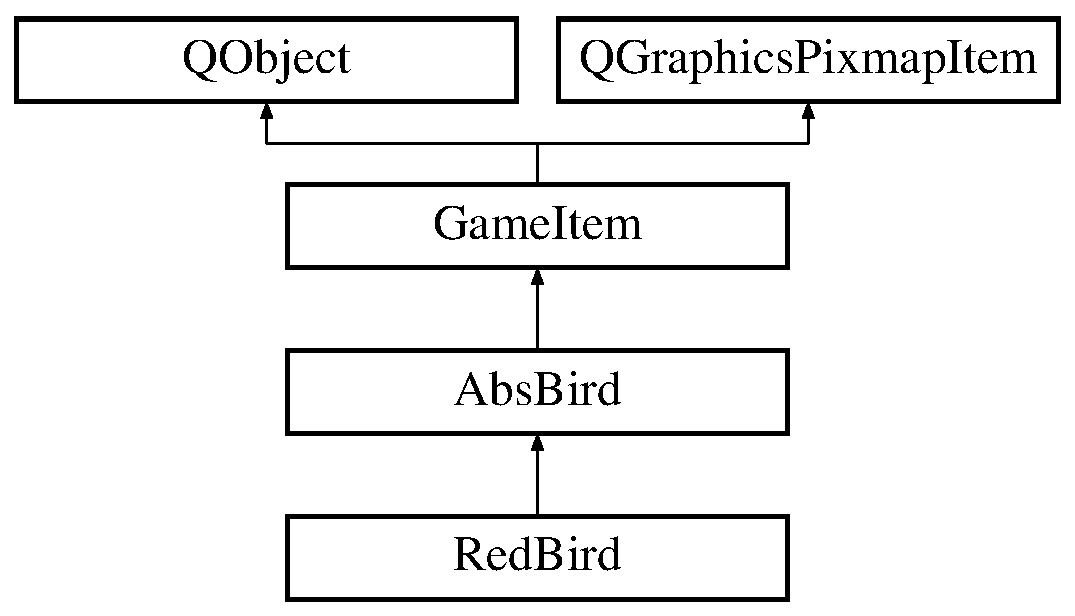
\includegraphics[height=4.000000cm]{classRedBird}
\end{center}
\end{figure}
\subsection*{Public Slots}
\begin{DoxyCompactItemize}
\item 
void {\bfseries update\+Pos} ()\hypertarget{classRedBird_abe6174521033b4aaf65d9ce66aaad0e6}{}\label{classRedBird_abe6174521033b4aaf65d9ce66aaad0e6}

\end{DoxyCompactItemize}
\subsection*{Public Member Functions}
\begin{DoxyCompactItemize}
\item 
{\bfseries Red\+Bird} (b2\+World $\ast$input\+World)\hypertarget{classRedBird_a4ce50ed34a0e94554a49b043060266e6}{}\label{classRedBird_a4ce50ed34a0e94554a49b043060266e6}

\end{DoxyCompactItemize}
\subsection*{Additional Inherited Members}


The documentation for this class was generated from the following files\+:\begin{DoxyCompactItemize}
\item 
Game\+Scene/\+Birds/Red\+Bird.\+h\item 
Game\+Scene/\+Birds/Red\+Bird.\+cpp\end{DoxyCompactItemize}

\hypertarget{classRestartButton}{}\section{Restart\+Button Class Reference}
\label{classRestartButton}\index{Restart\+Button@{Restart\+Button}}
Inheritance diagram for Restart\+Button\+:\begin{figure}[H]
\begin{center}
\leavevmode
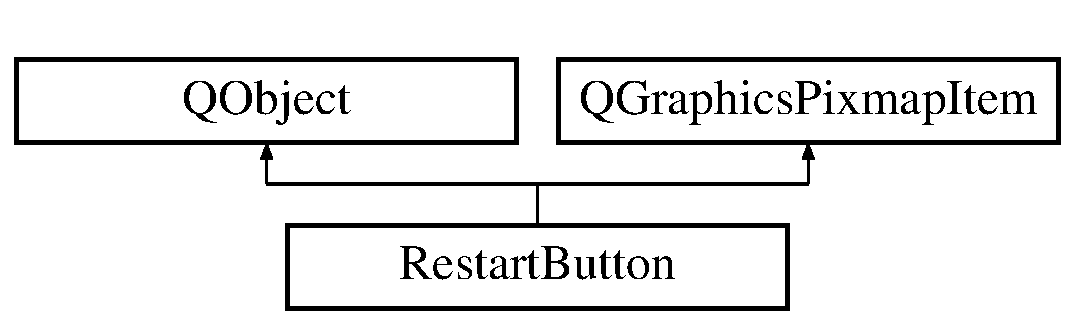
\includegraphics[height=2.000000cm]{classRestartButton}
\end{center}
\end{figure}
\subsection*{Signals}
\begin{DoxyCompactItemize}
\item 
void {\bfseries clicked} ()\hypertarget{classRestartButton_a9684d51fa4f34cbee2acfd80b41c95db}{}\label{classRestartButton_a9684d51fa4f34cbee2acfd80b41c95db}

\end{DoxyCompactItemize}
\subsection*{Public Member Functions}
\begin{DoxyCompactItemize}
\item 
void {\bfseries mouse\+Press\+Event} (Q\+Graphics\+Scene\+Mouse\+Event $\ast$event)\hypertarget{classRestartButton_ab67d3a7e6316985547eb6e02d4075bdb}{}\label{classRestartButton_ab67d3a7e6316985547eb6e02d4075bdb}

\item 
void {\bfseries hover\+Enter\+Event} (Q\+Graphics\+Scene\+Hover\+Event $\ast$event)\hypertarget{classRestartButton_adcad7b3dabbb5a645b13708a24e1cb26}{}\label{classRestartButton_adcad7b3dabbb5a645b13708a24e1cb26}

\item 
void {\bfseries hover\+Leave\+Event} (Q\+Graphics\+Scene\+Hover\+Event $\ast$event)\hypertarget{classRestartButton_ac71ab26cfefad7ee2214b110bb304138}{}\label{classRestartButton_ac71ab26cfefad7ee2214b110bb304138}

\end{DoxyCompactItemize}


The documentation for this class was generated from the following files\+:\begin{DoxyCompactItemize}
\item 
End\+Menu\+Scene/Restart\+Button.\+h\item 
End\+Menu\+Scene/Restart\+Button.\+cpp\item 
moc\+\_\+\+Restart\+Button.\+cpp\end{DoxyCompactItemize}

\hypertarget{classSingleshot}{}\section{Singleshot Class Reference}
\label{classSingleshot}\index{Singleshot@{Singleshot}}
Inheritance diagram for Singleshot\+:\begin{figure}[H]
\begin{center}
\leavevmode
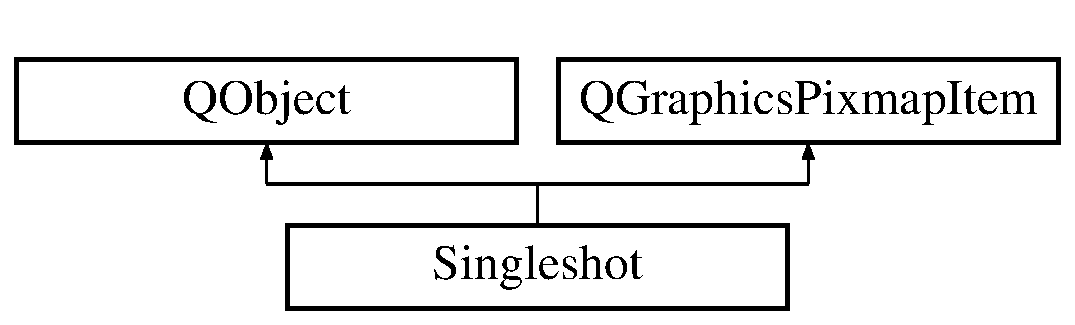
\includegraphics[height=2.000000cm]{classSingleshot}
\end{center}
\end{figure}
\subsection*{Public Slots}
\begin{DoxyCompactItemize}
\item 
void {\bfseries pull} (int x, int y)\hypertarget{classSingleshot_a0e2327fe3007b5f49aa6c09487bee84b}{}\label{classSingleshot_a0e2327fe3007b5f49aa6c09487bee84b}

\item 
void {\bfseries release} ()\hypertarget{classSingleshot_a3ad5aebe0a5930a39a4a94ffdb0872ff}{}\label{classSingleshot_a3ad5aebe0a5930a39a4a94ffdb0872ff}

\item 
void {\bfseries shorten} ()\hypertarget{classSingleshot_aca3cd8fc37f38197739cef321bcac79e}{}\label{classSingleshot_aca3cd8fc37f38197739cef321bcac79e}

\end{DoxyCompactItemize}
\subsection*{Signals}
\begin{DoxyCompactItemize}
\item 
void {\bfseries set\+New\+Bird} ()\hypertarget{classSingleshot_ad2d8b5788491f362189447b037ba148b}{}\label{classSingleshot_ad2d8b5788491f362189447b037ba148b}

\end{DoxyCompactItemize}
\subsection*{Public Attributes}
\begin{DoxyCompactItemize}
\item 
int {\bfseries forceX}\hypertarget{classSingleshot_ac2c993af762810642fb9e14050b98ff6}{}\label{classSingleshot_ac2c993af762810642fb9e14050b98ff6}

\item 
int {\bfseries forceY}\hypertarget{classSingleshot_ac5015fd8605425657701bad124210fb6}{}\label{classSingleshot_ac5015fd8605425657701bad124210fb6}

\end{DoxyCompactItemize}
\subsection*{Friends}
\begin{DoxyCompactItemize}
\item 
class {\bfseries Game\+Engine}\hypertarget{classSingleshot_a9ca20b077852bfc7b050d3a6a32d1a40}{}\label{classSingleshot_a9ca20b077852bfc7b050d3a6a32d1a40}

\end{DoxyCompactItemize}


The documentation for this class was generated from the following files\+:\begin{DoxyCompactItemize}
\item 
Game\+Scene/Singleshot.\+h\item 
Game\+Scene/Singleshot.\+cpp\item 
moc\+\_\+\+Singleshot.\+cpp\end{DoxyCompactItemize}

\hypertarget{classStick2__Hrz}{}\section{Stick2\+\_\+\+Hrz Class Reference}
\label{classStick2__Hrz}\index{Stick2\+\_\+\+Hrz@{Stick2\+\_\+\+Hrz}}
Inheritance diagram for Stick2\+\_\+\+Hrz\+:\begin{figure}[H]
\begin{center}
\leavevmode
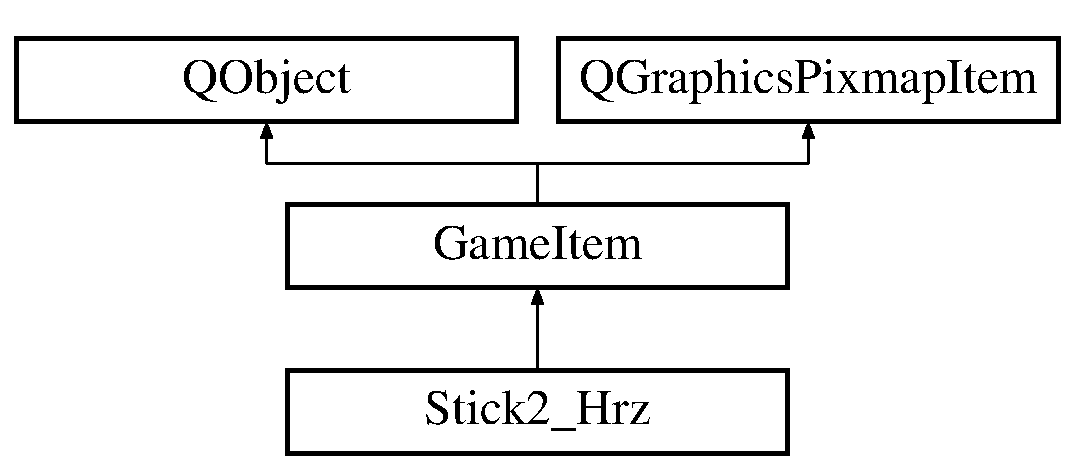
\includegraphics[height=3.000000cm]{classStick2__Hrz}
\end{center}
\end{figure}
\subsection*{Public Slots}
\begin{DoxyCompactItemize}
\item 
void {\bfseries update\+Pos} ()\hypertarget{classStick2__Hrz_a541f2a3db96c9a07ace5a584aa38f291}{}\label{classStick2__Hrz_a541f2a3db96c9a07ace5a584aa38f291}

\end{DoxyCompactItemize}
\subsection*{Public Member Functions}
\begin{DoxyCompactItemize}
\item 
{\bfseries Stick2\+\_\+\+Hrz} (b2\+World $\ast$input\+World, int inputX, int inputY)\hypertarget{classStick2__Hrz_ab48265110578343eb9c7394caccda625}{}\label{classStick2__Hrz_ab48265110578343eb9c7394caccda625}

\end{DoxyCompactItemize}
\subsection*{Additional Inherited Members}


The documentation for this class was generated from the following files\+:\begin{DoxyCompactItemize}
\item 
Game\+Scene/\+Random\+Items/Stick2\+\_\+\+Hrz.\+h\item 
Game\+Scene/\+Random\+Items/Stick2\+\_\+\+Hrz.\+cpp\end{DoxyCompactItemize}

\hypertarget{classStick2__Vtl}{}\section{Stick2\+\_\+\+Vtl Class Reference}
\label{classStick2__Vtl}\index{Stick2\+\_\+\+Vtl@{Stick2\+\_\+\+Vtl}}
Inheritance diagram for Stick2\+\_\+\+Vtl\+:\begin{figure}[H]
\begin{center}
\leavevmode
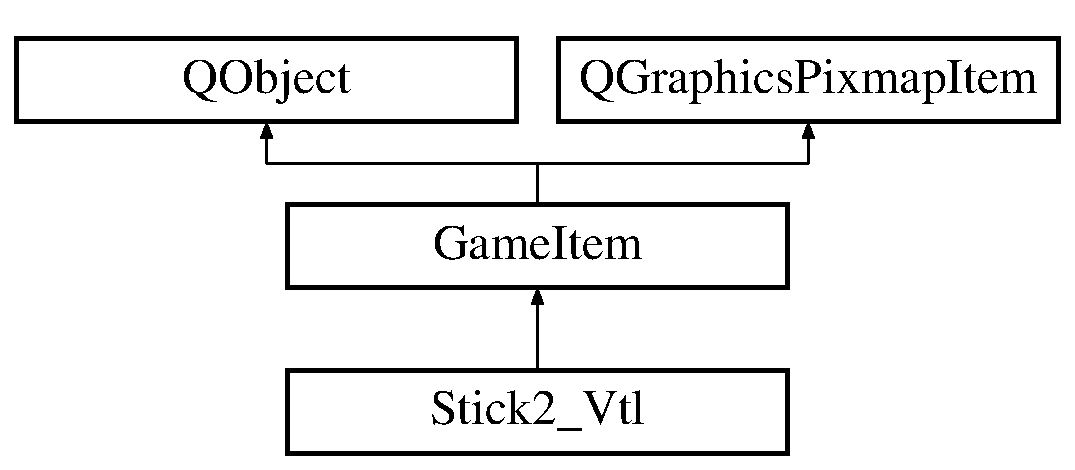
\includegraphics[height=3.000000cm]{classStick2__Vtl}
\end{center}
\end{figure}
\subsection*{Public Slots}
\begin{DoxyCompactItemize}
\item 
void {\bfseries update\+Pos} ()\hypertarget{classStick2__Vtl_ad9a849d2a3165de4a50f97fea13a570f}{}\label{classStick2__Vtl_ad9a849d2a3165de4a50f97fea13a570f}

\end{DoxyCompactItemize}
\subsection*{Public Member Functions}
\begin{DoxyCompactItemize}
\item 
{\bfseries Stick2\+\_\+\+Vtl} (b2\+World $\ast$input\+World, int inputX, int inputY)\hypertarget{classStick2__Vtl_a5487f43f916a017dde98cb8d93071291}{}\label{classStick2__Vtl_a5487f43f916a017dde98cb8d93071291}

\end{DoxyCompactItemize}
\subsection*{Additional Inherited Members}


The documentation for this class was generated from the following files\+:\begin{DoxyCompactItemize}
\item 
Game\+Scene/\+Random\+Items/Stick2\+\_\+\+Vtl.\+h\item 
Game\+Scene/\+Random\+Items/Stick2\+\_\+\+Vtl.\+cpp\end{DoxyCompactItemize}

\hypertarget{classStick__Hrz}{}\section{Stick\+\_\+\+Hrz Class Reference}
\label{classStick__Hrz}\index{Stick\+\_\+\+Hrz@{Stick\+\_\+\+Hrz}}
Inheritance diagram for Stick\+\_\+\+Hrz\+:\begin{figure}[H]
\begin{center}
\leavevmode
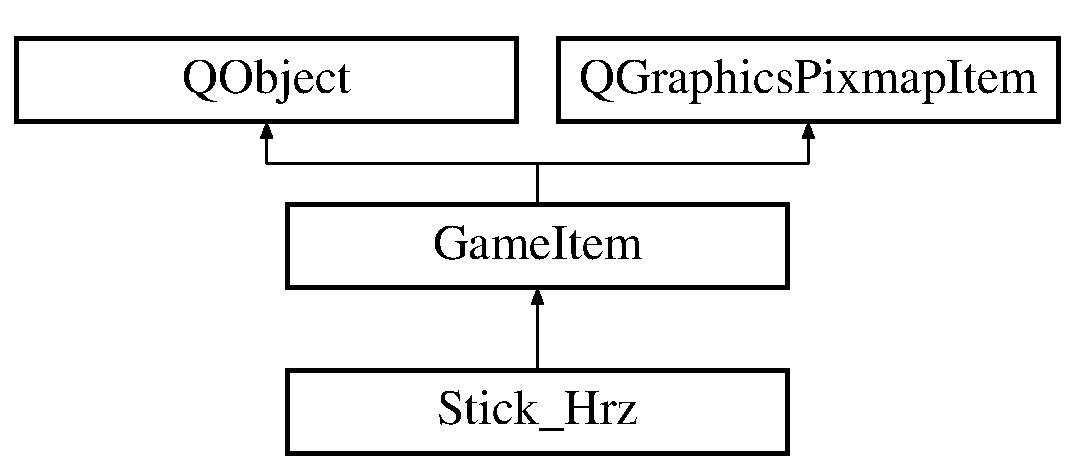
\includegraphics[height=3.000000cm]{classStick__Hrz}
\end{center}
\end{figure}
\subsection*{Public Slots}
\begin{DoxyCompactItemize}
\item 
void {\bfseries update\+Pos} ()\hypertarget{classStick__Hrz_ab39bc022ebe97d3fcb3e6830d86c71b1}{}\label{classStick__Hrz_ab39bc022ebe97d3fcb3e6830d86c71b1}

\end{DoxyCompactItemize}
\subsection*{Public Member Functions}
\begin{DoxyCompactItemize}
\item 
{\bfseries Stick\+\_\+\+Hrz} (b2\+World $\ast$input\+World, int inputX, int inputY)\hypertarget{classStick__Hrz_a5d36244f2d76d587bcb1dd6e5406e9f2}{}\label{classStick__Hrz_a5d36244f2d76d587bcb1dd6e5406e9f2}

\end{DoxyCompactItemize}
\subsection*{Additional Inherited Members}


The documentation for this class was generated from the following files\+:\begin{DoxyCompactItemize}
\item 
Game\+Scene/\+Random\+Items/Stick\+\_\+\+Hrz.\+h\item 
Game\+Scene/\+Random\+Items/Stick\+\_\+\+Hrz.\+cpp\end{DoxyCompactItemize}

\hypertarget{classStick__Vtl}{}\section{Stick\+\_\+\+Vtl Class Reference}
\label{classStick__Vtl}\index{Stick\+\_\+\+Vtl@{Stick\+\_\+\+Vtl}}
Inheritance diagram for Stick\+\_\+\+Vtl\+:\begin{figure}[H]
\begin{center}
\leavevmode
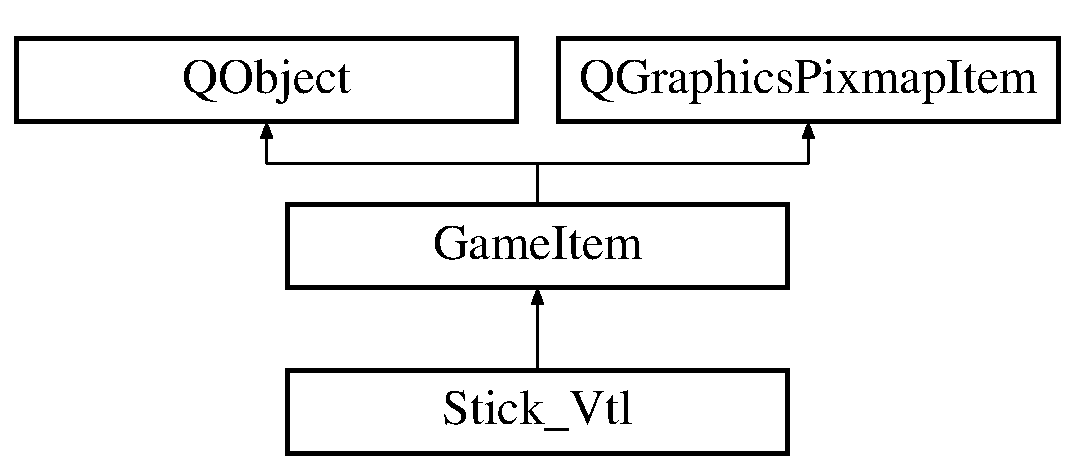
\includegraphics[height=3.000000cm]{classStick__Vtl}
\end{center}
\end{figure}
\subsection*{Public Slots}
\begin{DoxyCompactItemize}
\item 
void {\bfseries update\+Pos} ()\hypertarget{classStick__Vtl_a92838d5c7c74ecd6843a3060c28ed0d0}{}\label{classStick__Vtl_a92838d5c7c74ecd6843a3060c28ed0d0}

\end{DoxyCompactItemize}
\subsection*{Public Member Functions}
\begin{DoxyCompactItemize}
\item 
{\bfseries Stick\+\_\+\+Vtl} (b2\+World $\ast$input\+World, int inputX, int inputY)\hypertarget{classStick__Vtl_a8b0b4c1ecc362b676b223ffe37fea00d}{}\label{classStick__Vtl_a8b0b4c1ecc362b676b223ffe37fea00d}

\end{DoxyCompactItemize}
\subsection*{Additional Inherited Members}


The documentation for this class was generated from the following files\+:\begin{DoxyCompactItemize}
\item 
Game\+Scene/\+Random\+Items/Stick\+\_\+\+Vtl.\+h\item 
Game\+Scene/\+Random\+Items/Stick\+\_\+\+Vtl.\+cpp\end{DoxyCompactItemize}

\hypertarget{classYellowBird}{}\section{Yellow\+Bird Class Reference}
\label{classYellowBird}\index{Yellow\+Bird@{Yellow\+Bird}}
Inheritance diagram for Yellow\+Bird\+:\begin{figure}[H]
\begin{center}
\leavevmode
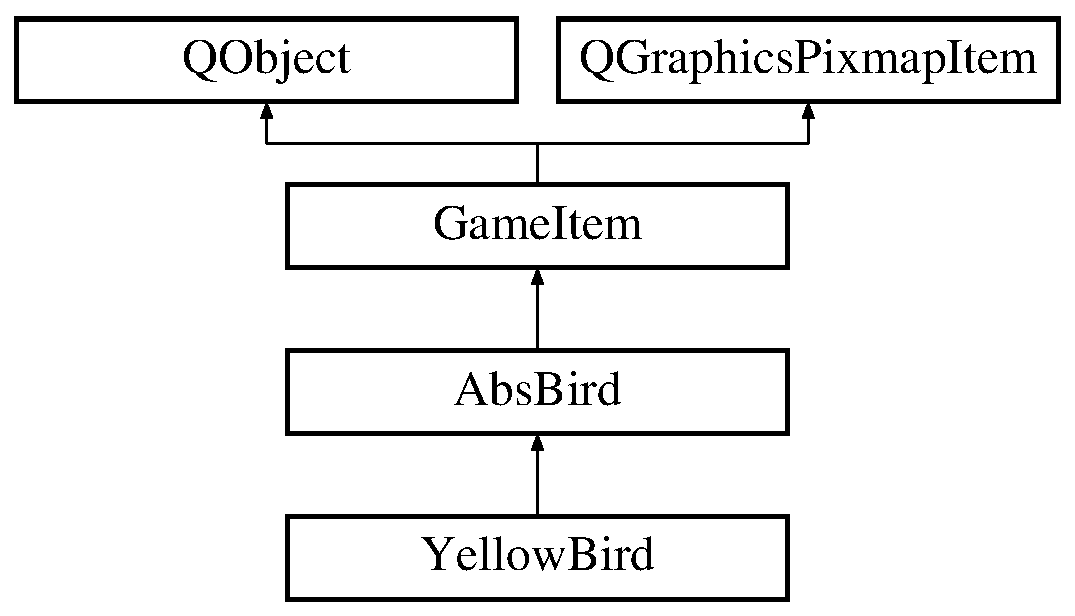
\includegraphics[height=4.000000cm]{classYellowBird}
\end{center}
\end{figure}
\subsection*{Public Slots}
\begin{DoxyCompactItemize}
\item 
void {\bfseries update\+Pos} ()\hypertarget{classYellowBird_a6c3ceb34f93c373fdb708242b187c61f}{}\label{classYellowBird_a6c3ceb34f93c373fdb708242b187c61f}

\item 
void {\bfseries special\+Ability} ()\hypertarget{classYellowBird_ac0d2338bebfc57cc7b524d185bbfe721}{}\label{classYellowBird_ac0d2338bebfc57cc7b524d185bbfe721}

\end{DoxyCompactItemize}
\subsection*{Public Member Functions}
\begin{DoxyCompactItemize}
\item 
{\bfseries Yellow\+Bird} (b2\+World $\ast$input\+World)\hypertarget{classYellowBird_ac32d1c19aff515544d98cbe08adfc4c2}{}\label{classYellowBird_ac32d1c19aff515544d98cbe08adfc4c2}

\end{DoxyCompactItemize}
\subsection*{Additional Inherited Members}


The documentation for this class was generated from the following files\+:\begin{DoxyCompactItemize}
\item 
Game\+Scene/\+Birds/Yellow\+Bird.\+h\item 
Game\+Scene/\+Birds/Yellow\+Bird.\+cpp\end{DoxyCompactItemize}

%--- End generated contents ---

% Index
\backmatter
\newpage
\phantomsection
\clearemptydoublepage
\addcontentsline{toc}{chapter}{Index}
\printindex

\end{document}
